%
% Dataontwerp
%

\chapter{Dataontwerp}

\section{Entity-relationship model}
\begin{figure}[h!]
	\centering
		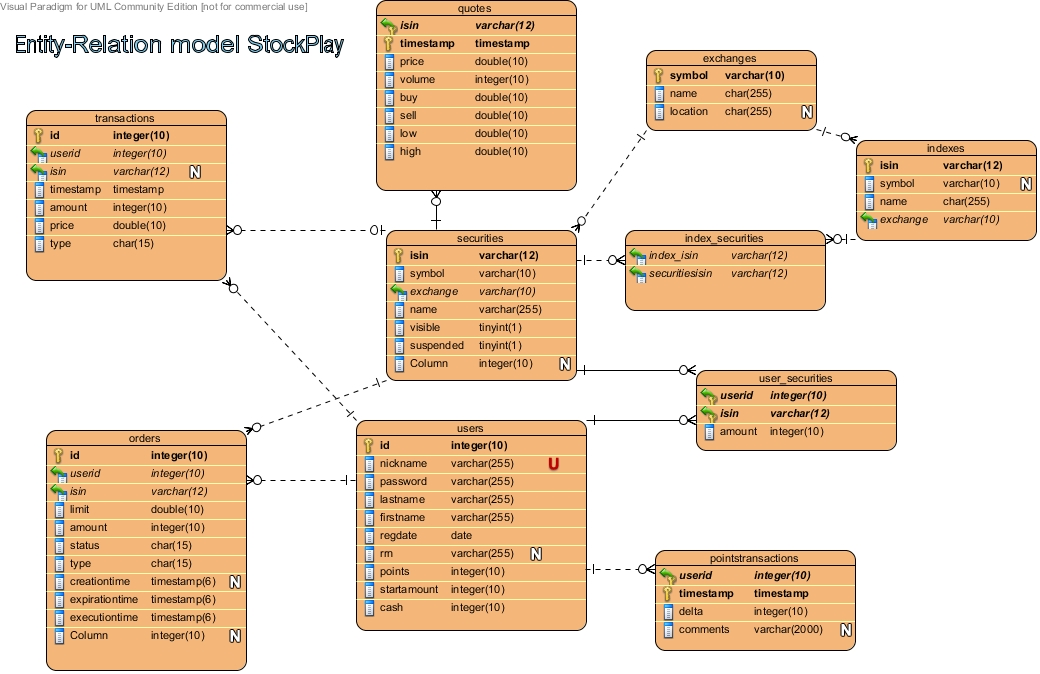
\includegraphics[width=\textwidth]{images/realisatie/ER_Diagram}
	\caption{Het entity-relationship model.}
\end{figure}

\section{Afscheiding datatoegang}

Door het gebruik van een aparte backend, wordt rechtstreekse toegang tot de effectieve data verhinderd. Zo kunnen we doorgedreven controles en verificatie van de ingegeven data toepassen, alsook eventuele optimalisaties doorvoeren. Onderstaand diagram illustreert de samenwerking van de componenten in kwestie:

\begin{figure}[h!]
	\centering
		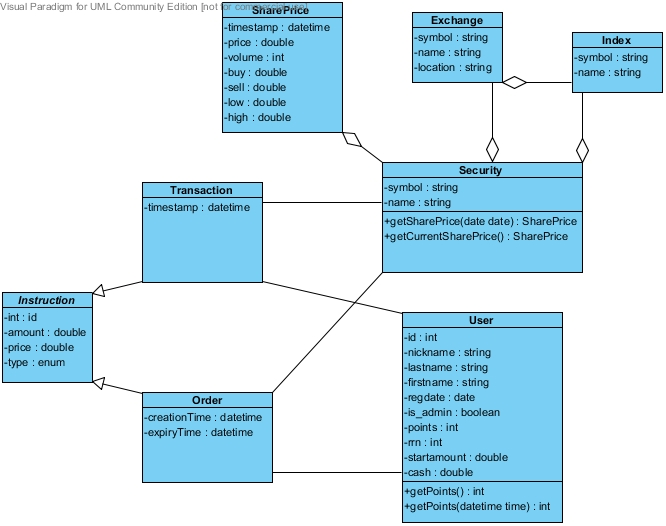
\includegraphics[width=0.5\textwidth]{images/realisatie/Class_Diagram}
	\caption{Overzicht van de werking van de backend.}
\end{figure}

\section{Triggers}

% Configureren van codefragmenten
\lstset{language=SQL,style=SQL}

In de tabel ``users'' bevinden zich twee kolommen met redundante informatie: cash en points. De tabel ``user\_securities'' is zelfs in zijn geheel redundant. Om te voorkomen dat er inconsistentie zou optreden binnen de database, werd besloten van triggers gebruik te maken.

De cashpositie van een speler verandert wanneer er een transactie op zijn account wordt geregistreerd. Dit gebeurd wanneer er een rij wordt toegevoegd aan de ``transactions''-tabel. Dan wordt door middel van een trigger de cashpositie van de gebruiker, alsook de wijziging in de hoeveelheid effecten die hij bezit geregistreerd met behulp van de trigger te zien in codefragment \ref{code:data:trig_cash}.

\begin{code}
\begin{lstlisting}
create or replace
TRIGGER UPDATECASH
AFTER INSERT OR UPDATE ON TRANSACTIONS 
REFERENCING OLD AS old NEW as new
FOR EACH ROW 
DECLARE
  us_exists number;
BEGIN
  SELECT count(1) INTO us_exists FROM user_securities us WHERE us.userid = coalesce(:new.userid, :old.userid) AND us.isin = coalesce(:new.isin,:old.isin);
  IF coalesce(:new.type, :old.type) = 'SELL' THEN
      UPDATE users u SET u.cash=u.cash+coalesce(:new.price*:new.amount,0)-coalesce(:old.price*:old.amount,0) WHERE u.id=coalesce(:new.userid,:old.userid);
      IF us_exists > 0 THEN
            UPDATE user_securities us SET us.amount=us.amount-coalesce(:new.amount,0)+coalesce(:old.amount,0) WHERE us.userid = coalesce(:new.userid, :old.userid) AND us.isin = coalesce(:new.isin,:old.isin);
      ELSE
            INSERT INTO user_securities (userid, isin, amount) VALUES( coalesce(:new.userid, :old.userid), coalesce(:new.isin,:old.isin), -coalesce(:new.amount, :old.amount));
      end IF;
  ELSE
      UPDATE users u SET u.cash=u.cash-coalesce(:new.price*:new.amount,0)+coalesce(:old.price*:old.amount,0) WHERE u.id=coalesce(:new.userid,:old.userid);
             if us_exists > 0 THEN
            UPDATE user_securities us SET us.amount=us.amount+coalesce(:new.amount,0)-coalesce(:old.amount,0) WHERE us.userid = coalesce(:new.userid, :old.userid) AND us.isin = coalesce(:new.isin,:old.isin);
      ELSE
            INSERT INTO user_securities (userid, isin, amount) VALUES( coalesce(:new.userid, :old.userid), coalesce(:new.isin,:old.isin), coalesce(:new.amount, :old.amount));
      end IF;
  end IF;
END;
\end{lstlisting}
\caption{Trigger verantwoordelijk voor het updaten van de cashpositie van gebruikers.}
\label{code:data:trig_cash}
\end{code}

Een transactie is ook niet altijd mogelijk: als een speler een te lage cashpositie bezit, of te weinig effecten om te kunnen verkopen, dan kan een transactie niet doorgaan. Dit wordt gecontroleerd door de trigger die te zien is in codefragment \ref{code:data:trig_transacties}.

\begin{code}
\begin{lstlisting}
create or replace
TRIGGER CHECKTRANSACTION
BEFORE INSERT OR UPDATE ON TRANSACTIONS 
FOR EACH ROW 
DECLARE
  money_user number;
  has_sec number;
  amount_owned number;
BEGIN
  if :new.price < 0 or :new.amount < 0 then
    raise_application_error(-20000, 'Price and amount should ALWAYS be positive!');
  end if;
    
  if (:new.type = 'BUY') then
      select cash into money_user from users u WHERE u.id = :new.userid;
    if ((money_user - (:new.price*:new.amount)) < 0) then
      raise_application_error(-20001, 'User doesnt have enough cash!');
    end if;

  elsif (:new.type = 'SELL') then
    select count(1) into has_sec from user_securities us where us.userid = :new.userid and us.isin = :new.isin;
    
    if(has_sec > 0) then 
    
      select amount into amount_owned from user_securities us where us.userid = :new.userid and us.isin = :new.isin;
      if (:new.amount > amount_owned) then
        raise_application_error(-20001, 'User doesnt have enough securities of that ISIN!');
      end if;
    else
        raise_application_error(-20001, 'User doesnt have securities of that ISIN!');
    end if;
  end if;
END;
\end{lstlisting}
\caption{Trigger verantwoordelijk voor het controlern van transacties.}
\label{code:data:trig_transacties}
\end{code}


Wijzingen in punten bij een speler wordt geregistreerd in de tabel ``pointtransactions'', dat laat toe om een meer verfijnde klassementen op te stellen (dagklassement, weekklassement, maandklassement, ...). Het totale aantal punten wordt berekend met behulp van een trigger in de ``users''-tabel, wiens code vermeld staat in codefragment \ref{code:data:trig_punten}.

\begin{code}
\begin{lstlisting}
create or replace
TRIGGER UPDATEPOINTS
AFTER INSERT OR UPDATE OR DELETE ON POINTSTRANSACTIONS 
REFERENCING OLD AS old NEW as new
FOR EACH ROW 
BEGIN
  UPDATE users u SET u.points=coalesce(u.points,0)+coalesce(:new.delta,0)-coalesce(:old.delta,0) WHERE u.id=coalesce(:new.userid,:old.userid);
END;
\end{lstlisting}
\caption{Trigger verantwoordelijk voor het berekenen van het puntentotaal.}
\label{code:data:trig_punten}
\end{code}

%
% Procedureontwerp
%

\chapter{Backend}

\section{Data Access Objects}

Een probleem bij de huidige implementatie is de relatief grote ``afstand'' tussen de lineaire voorstelling van data in een database en de rijkere voorstelling van data in objecten. Dit omdat er andere manieren worden gebruikt om overerving, relaties tussen data, enzovoort, voor te stellen. Dit probleem is in de literatuur beter bekend als de ``object-relational impedance mismatch''. Een veelgebruikte oplossing is die van de Object-Relational Mapping-tools, waarvan het gebruik voor deze bachelorproef uitgesloten werd.. Daarom werd er op zoek gegaan naar andere conceptuele ide\"en die gebruikt konden worden, en uiteindelijk werd er gekozen voor het gebruik van het ``Data Access Object''-pattern.

Het DAO-pattern koppelt op een eenvoudige manier de businesslogica los van het mechanisme dat de data permanent opslaat. Dit zorgt ervoor dat de businesslogica meer robuust en flexibeler is wanneer er wijzigingen zouden optreden in de manier waarop de data wordt opgeslagen.

Een data access object voorziet in zijn meest eenvoudige vorm 4 operaties: het ophalen, aanmaken, wijzigen en verwijderen van een object. Dit wordt grotendeels weerspiegeld in de gebruikte interface bij dit project:

\lstset{language=Java,style=Java}
\begin{lstlisting}
public interface GenericDAO<T, ID> {

    public T findById(ID id);
    public Collection<T> findByFilter(Filter iFilter);
    public Collection<T> findAll();

    public boolean update(T entity);
    public int create(T entity);
    public boolean delete(T entity);
}
\end{lstlisting}

De objecten die de eigenlijke data bevatten worden de ``Data Transfer Objects'' (DTO's) genoemd. De businesslogica kan de data in deze objecten aanpassen zonder dat dit gevolgen heeft op de persistente data. Pas als het DTO weer wordt doorgegeven aan het DAO, wordt de persistente data gewijzigd. Dit maakt het gebruik van dit pattern erg geschikt voor onze backend, waar de eigenlijke wijzigingen van de data niet op niveau van de backend gebeuren, maar wel door de modules die op de backend inhaken. Deze DTO's zijn namelijk erg ``licht'' omdat ze enkel gebruikt worden om data voor te stellen, en kunnen dus gemakkelijk via het XML-RPC-protocol verstuurd worden.

\section{XML-RPC interface}

Zoals vermeld bij het technisch ontwerp, gebruiken we het XML-RPC protocol als communicatiemiddel tussen de backend en zijn interfaces. Hiertoe moesten we de set aan functies vastleggen die een client kan uitvoeren, en de bijhorende signatuur documenteren.

Aangezien XML-RPC geen ondersteuning biedt voor namespaces of andere vormen van functieorganisatie, hanteren we zelf een mechanisme om dit te bekomen: een methode-naam bestaat altijd uit meerdere delen, gescheiden door een punt. De delen voor het scheidingsteken duiden de ``klasse'', het deel erna de methode die we willen oproepen.
Zo delen we de backend op in de volgende drie primaire klassen:
\begin{itemize_compact}
\item{\emph{System}: functionaliteit voor beheer en de statusinformatie van het systeem.}
\item{\emph{User}: beheer van gebruikers en ophalen gebruikersinformatie.}
\item{\emph{Finance}: functionaliteit gerelateerd aan het beurswezen.}
\end{itemize_compact}

\subsection{Algemene foutcodes}

De XML-RPC specificatie biedt ook ondersteuning voor foutberichten, in de form van een bericht met een $<$fault$>$ tag. Die tag moet steeds twee $<$member$>$ tags bevatten, namelijk een foutcode $<$faultCode$>$ van het integer type, en een foutbericht $<$faultString$>$ van het string type.

De mogelijke foutberichten die de backend kan opwerpen, zijn onderverdeeld in verschillende klassen. Bij elke klasse valt de foutcode dan in een specifiek vooraf gedefini\"eerd bereik, zodat client-software eenvoudig kan detecteren om welk soort fout het gaat. De exacte foutcode, eveneens op voorhand vastgelegd, bepaald vervolgens welke fout er opgeworpen is. Zie tabel \ref{tbl:real:xmlrpc:fouten} voor de mogelijke fouten.
Bij elk type fout gaat zo een standaard foutbericht gepaard, maar de backend-ontwikkelaar kan die eventueel vervangen door een meer specifieke foutmelding.

Om meer informatie over een specifieke fout te bekomen, moet naar de log van de backend gekeken worden. Daar wordt telkens de exacte ``stacktrace'' vermeld, zodat de fout eenvoudig te verhelpen wordt. Een speciaal type fout tenslotte, is de ``internal exception''. Deze treedt op wanneer een exceptie onverwacht optrad, en dus niet in een correcte try-catch blok opgevangen werd.

\begin{table}
\begin{tabular}{| c p{4cm} p{7cm} |}
	\hline
	Foutcode & Foutbericht & Opmerking \\
	\hline
	
	0 & Internal Failure & Een ``untrapped exception'', niet opgevangen door een correcte try-catch clause. \\
	\hline
	
	$[1-10[$ & \emph{Subsystem failures.} & \\
	1 & Database Failure & Er is een probleem met de database (onbeschikbaar, corrupt, ...), zie de log voor meer details. \\
	2 & Scraper Failure & Er is een probleem met de scraper (onbeschikbaar, uitgevallen, ...), zie de log voor meer details. \\
	\hline
	
	$[10-20[$ & \emph{Service exceptions.} & \\
	10 & Service Unavailable & De backend kan tijdelijk niet gebruikt worden (werkzaamheden, overloaded, ...). \\
	11 & Unauthorized & De huidige gebruiker is niet geautoriseerd om de functie in kwestie uit te voeren. \\
	12 & Invalid Credentials & De poging om aan te melden is mislukt, wegens een foutieve gebruikersnaam en wachtwoord combinatie. \\
	13 & Session Corrupt & De meegeleverde sessie is niet geregistreerd in de backend (verlopen of corrupt). \\
	14 & Not Enough Information & Er is niet genoeg informatie om het object aan te maken (meestal betekent dit dat er een veld in de meegeleverde struct ontbreekt). \\
	\hline
	
	$[20-30[$ & \emph{Invocation issues.} & \\
	20 & Version Not Supported & De client gebruikt een foutief communicatieprotocol. \\
	21 & Not Found & Er is geen methode gevonden met die naam, verifieer de schrijfwijze en de klasse. \\
	22 & Bad Request & Probleem met de parameters, controleer de documentatie van de methode. \\
	23 & Non Existing Entity & Het item dat je opvroeg bestaat niet \\
	24 & Pre Existing Entity & Er bestaat reeds zo'n item \\
	25 & Read Only Key & Er is een aanvraag gedaan om een key aan te passen die niet aangepast mag worden \\
	26 & Key does not exist & Er is een aanvraag gedaan om een key aan te passen die niet bestaat \\
	\hline

	$[30-40[$ & \emph{Filter issues.} & \\
	31 & Filter Failure & Er is een probleem met de doorgegeven filter, controleer deze. \\
	32 & Debug Failure & De backend is er niet in geslaagd een debug-AST te genereren van de filter, is de benodigde software ge\"installeerd? \\
	33 & Filter Failure & De backend slaagde er niet in twee filters samen te voegen om een resultaatset-reductie te bekomen. \\
	
	\hline
\end{tabular}
\caption{Mogelijke fouten binnen het backend-protocol}
\label{tbl:real:xmlrpc:fouten}
\end{table}

\subsection{Authenticatie en autorisatie}

Aangezien het XML-RPC protocol gebruik maakt van het HTTP-protocol, waren we van plan om diens functionaliteit gebruiken om authenticatie te bekomen. Daartoe zouden we gebruik maken van \emph{basic authentication}, waarbij de client indien gevraagd een gebruikersnaam en wachtwoord naar de server doorstuurd. Normaal zou dit geen extra code te weeg gebracht hebben en zouden we volledig op de authenticatiemogelijkheden van het HTTP protocol kunnen berusten.

Deze denkpiste gaf echter enkele problemen. Vooreerst is het sterk onveilig aangezien het wachtwoord continu in (quasi) plaintext doorgestuurd wordt. Het maakt echter verfijnde autorisatie moeilijk, tenzij we voor elk authenticatie-niveau een aparte URL zouden voorzien. Daarom hebben we gekozen om gebruik te maken van een eigen authenticatie-laag, waarbij een XML-RPC functie gebruikt wordt om de gebruiker aan te melden (dit in tegenstelling tot het gebruik maken van de HTTP laag). Na aanmelding geeft de functie in kwestie een sessie-ID terug, die een sessie serverside linkt aan een specifieke gebruiker. Zo kunnen we, opnieuw binnenin de XML-RPC laag, controleren of een gebruiker wel correct aangemeld is en heel dynamisch requests toelaten of weigeren. Dit is gebaseerd op een flexibel rechten-systeem, waarbij elke gebruiker in de database gelinkt wordt aan een rol die bepaalde rechten toekent.

Om de veiligheid te verhogen gebruiken we verschillende technieken. Eerst en vooral is de sessie tijdelijk, en worden ongebruikte sessie-keys regelmatig ge�nvalideerd. Ook hebben we het moeilijk gemaakt om sessie-keys te genereren, door ze op een unieke manier te linken aan data die enkel de gebruiker zelf kent (zijn wachtwoord). Om het tenslotte ook moeilijk te maken om een sessie-key te linken aan een gebruiker, implementeren we in onze sessie-hash een variabele seed.

Authenticatie en autorisatie gaat ook gepaard met een specifieke set aan mogelijke foutboodschappen. Allemaal geklasseerd binnen de Service Bezwaren zijn de volgende subtypes mogelijk: ``Invalid Credentials'' wanneer het authenticeren mislukt is, ``Unauthorized'' wanneer een gebruiker niet geautoriseerd is tot het gebruik van een bepaalde functie en tenslotte ``Session Corrupt'' wanneer een gespecificeerde sessie ongeldig blijkt te zijn (zie tabel \ref{tbl:real:xmlrpc:fouten}).

De mogelijke autorisatieniveau's zijn beschreven in tabel \ref{tbl:real:xmlrpc:autorisatie}. Hoewel een administrator deze bij gebruikers manueel kan aanpassen, onderscheiden we toch volgende categorie\"en:
\begin{itemize_compact}
\item{Gast}
\item{Speler}
\item{Administrator}
\item{Scraper}
\item{Puntenmanager}
\item{Transactiemanager}
\item{AI}
\end{itemize_compact}

\begin{table}
\begin{tabular}{| c p{7cm} |}
	\hline
	Autorisatie-niveau & Beschrijving \\
	\hline
	
	BACKEND\_ADMIN & Administrator rechten voor methodes betreffende de backend. \\
	DATABASE\_ADMIN & Administrator rechten voor methodes betreffende de database. \\
	SCRAPER\_ADMIN & Administrator rechten voor methodes betreffende de scraper. \\
	POINTS\_ADMIN & Administrator rechten voor methodes betreffende het puntenbeheer. \\
	TRANSACTION\_ADMIN & Administrator rechten voor methodes betreffende het transactie-beheer. \\
	
	SECURITY\_UPDATE & Toegang tot methodes die effecten updaten (toevoegen van quotes). \\
	SECURITY\_CREATE & Toegang tot methodes die nieuwe effecten aanmaken. \\
	SECURITY\_REMOVE & Toegang tot methodes die effecten verwijderen. \\
	SECURITY\_MODIFY & Toegang tot methodes die effecten wijzigen. \\
	
	USER\_REMOVE & Toegang tot methodes die gebruikers verwijderen. \\
	
	LOGGEDIN & Standaard-recht voor ingelogde gebruikers. \\
	NONE & Standaard recht voor iedereen (ook gasten). \\
	
	\hline
\end{tabular}
\caption{Autorisatieniveau's binnen het backend-protocol.}
\label{tbl:real:xmlrpc:autorisatie}
\end{table}

\subsection{System klasse}

Deze klasse biedt de client mogelijkheden om het systeem te beheren. Zoals het ophalen van informatie, wijzigen van configuraties, en (her)starten of stoppen van bepaalde subsystemen.

\subsubsection{Backend subklasse}

\function{Backend.Status}
	{ status van de backend ophalen }
	{ geen }
	{ integer die de status beschrijft:
		\begin{itemize_compact}
		\item{0: maintenance-mode}
		\item{1: functioneert normaal}
		\end{itemize_compact} }
	{ BACKEND\_ADMIN }

\function{Backend.Stats}
	{ backend-statistieken ophalen }
	{ geen }
	{ struct met statistieken:
		\begin{itemize_compact}
		\item{users: aantal gebruikers online}
		\item{req: aantal verwerkte XML-RPC requests sinds de start van de backend}
		\item{uptime: hoe lang de backend al draait}
		\end{itemize_compact} }
	{ BACKEND\_ADMIN }

\function{Backend.Restart (NIET GE\"IMPLEMENTEERD)}
	{ de backend opnieuw opstarten }
	{ geen }
	{ bool die indiceert of de actie succesvol was }
	{ BACKEND\_ADMIN }

\function{Backend.Stop (NIET GE\"IMPLEMENTEERD)}
	{ de backend stoppen }
	{ geen }
	{ bool die indiceert of de actie succesvol was }
	{ BACKEND\_ADMIN }

\function{Backend.ClearCache}
	{ de backend cache legen, zodat die opnieuw alle data uit zijn datalagen dient op te halen}
	{ geen }
	{ bool die indiceert of de actie succesvol was }
	{ BACKEND\_ADMIN }


\subsubsection{Database subklasse}

\function{Database.Status}
	{ informatie van de database ophalen }
	{ geen }
	{ integer die status beschrijft:
		\begin{itemize_compact}
		\item{0: er kon geen verbinding naar de databank gelegd worden}
		\item{1: succesvol verbonden met de database}
		\end{itemize_compact} }
	{ DATABASE\_ADMIN }

\function{Database.Stats}
	{ database-statistieken ophalen. Dit zijn de statistieken geleverd door de databank zelf, ze zijn dus niet beperkt tot acties ondernomen door de backend }
	{ geen }
	{ struct met statistieken:
		\begin{itemize_compact}
		\item{uptime: hoe lang de databank al draait}
		\item{rate: aantal transacties per seconde}
		\end{itemize_compact} }
	{ DATABASE\_ADMIN }


\subsubsection{Scraper subklasse}

\function{Scraper.Status (NIET GE\"IMPLEMENTEERD)}
	{ status van de scraper ophalen }
	{ geen }
	{ integer die status beschrijft:
		\begin{itemize_compact}
		\item{0: niet geactiveerd}
		\item{1: inactief}
		\item{2: bezig met data-mining}
		\end{itemize_compact} }
	{ SCRAPER\_ADMIN }

\function{Scraper.Stats (NIET GE\"IMPLEMENTEERD)}
	{ scraper-statistieken ophalen }
	{ geen }
	{ struct met statistieken:
		\begin{itemize_compact}
		\item{executes: aantal voltooide plugin-uitvoeringen}
		\item{uptime: hoe lang de scraper al draait}
		\item{traffic: hoeveelheid data verzonden en ontvangen}
		\item{plugins: aantal geactiveerde plugins}
		\item{securities: aantal beschikbare effecten}
		\item{exchanges: aantal beschikbare beurzen}
		\item{indexes: aantal beschikbare indexen}
		\item{delay: tijd tot de volgende plugin-uitvoering}
		\item{memory: geheugengebruik}
		\end{itemize_compact} }
	{ SCRAPER\_ADMIN }

\function{Scraper.Restart (NIET GE\"IMPLEMENTEERD)}
	{ de scraper herstarten }
	{ geen }
	{ bool die indiceert of de actie succesvol was }
	{ SCRAPER\_ADMIN }

\function{Scraper.Stop (NIET GE\"IMPLEMENTEERD)}
	{ de scraper permanent stilleggen }
	{ geen }
	{ bool die indiceert of de actie succesvol was }
	{ SCRAPER\_ADMIN }

\subsection{User klasse}

Hier vindt men de nodige methodes terug om gebruikers te beheren. Dit is echter niet beperkt tot de administrator: ook gebruikers zelf kunnen hun eigen profiel (in beperktere mate) beheren.

\function{Hello}
	{ protocolcontrole uitvoeren }
	{ de naam van de applicatie (string), en het nummer van de protocolimplementatie (int) }
	{ een boolean die aangeeft of de actie al dan niet gelukt is, of een exceptie indien de vermelde protocolversie niet ondersteund wordt }
	{ NONE }
	
\function{Validate}
	{ controleren van user credentials en genereren van een sessie-ID }
	{ de gebruikersnaam (string) en wachtwoord (string) }
	{ een sessie-ID voor verder gebruik, of een exceptie indien het aanmelden mislukt is }
	{ NONE }
		
\function{CreateSessionForUser}
	{ manueel een sessie cre\"eren voor verder gebruik }
	{ de user-id waarvoor een sessie moet gecre\"eerd worden }
	{ een sessie-ID voor verder gebruik }
	{ BACKEND\_ADMIN }

\function{List}
	{ lijst met publieke informatie opvragen van de gebruikers }
	{ een filter om gebruikers te selecteren, met de volgende mogelijke sleutels:
		\begin{itemize_compact}
		\item{id: de ID van de gebruiker}
		\item{nickname: gebruikersnaam}
		\item{firstname: de voornaam van de gebruiker}
		\item{lastname: de achternaam van de gebruiker}
		\item{rrn: het rijksregisternummer van de gebruiker}
		\item{email: het e-mailadres van de gebruiker}
		\item{regtime: datum van registratie}
		\item{cash: de hoeveelheid cash die de gebruiker effectief bezit}
		\item{points: aantal behaalde punten}
		\end{itemize_compact} }
	{ een lijst met oppervlakkige gebruikersinformatie (in de vorm van een struct):
		\begin{itemize_compact}
		\item{id: gebruikers-id}
		\item{nickname: gebruikersnaam}
		\item{cash: de hoeveelheid cash die de gebruiker effectief bezit}
		\item{regdate: datum van registratie}
		\item{startamount: het kapitaal waarmee de gebruiker begonnen is}
		\item{points: aantal behaalde punten}
		\item{role: een verwijzing naar de rollen die de gebruiker beoefent}
		\end{itemize_compact} }
	{ NONE }

\function{Details}
	{ lijst met publieke informatie opvragen van een gebruiker }
	{ een filter om gebruikers te selecteren, zie de List functie }
	{ een lijst met gedetailleerde gebruikersinformatie (in de vorm van een struct):
			\begin{itemize_compact}
			\item{id: gebruikers-id}
			\item{nickname: gebruikersnaam}
			\item{firstname: de voornaam van de gebruiker}
			\item{lastname: de achternaam van de gebruiker}
			\item{email: het e-mailadres van de gebruiker}
			\item{cash: de hoeveelheid cash die de gebruiker effectief bezit}
			\item{regdate: datum van registratie}
			\item{rrn: het rijksregisternummer van de gebruiker}
			\item{startamount: het kapitaal waarmee de gebruiker begonnen is}
			\item{points: aantal behaalde punten}
			\item{role: een verwijzing naar de rollen die de gebruiker beoefent}
			\end{itemize_compact} }
	{ BACKEND\_ADMIN }
	
\function{Details}
	{ publieke informatie opvragen van de gebruiker zelf }
	{ geen (de filter wordt impliciet geconfigureerd op een selectie van details van de huidige gebruiker) }
	{ idem als Details aanroep met een filter }
	{ LOGGEDIN }

\function{Create}
	{ aanmaken van een nieuwe gebruiker }
	{ struct met de gebruikersinformatie:
		\begin{itemize_compact}
		\item{nickname: gebruikersnaam}
		\item{firstname: de voornaam van de gebruiker}
		\item{lastname: de achternaam van de gebruiker}
		\item{email: het e-mailadres van de gebruiker}
		\item{rrn: het rijksregisternummer van de gebruiker}
		\item{role: een verwijzing naar de rollen die de gebruiker beoefent}
		\end{itemize_compact} }
	{ id van de aangemaakte gebruiker }
	{ NONE }

\function{Modify}
	{ wijzigen van een bestaande gebruiker }
	{ een filter die gebruikers selecteert, en een struct met de te-wijzigen gebruikersinformatie:
		\begin{itemize_compact}
			\item{nickname: gebruikersnaam}
			\item{firstname: de voornaam van de gebruiker}
			\item{lastname: de achternaam van de gebruiker}
			\item{email: het e-mailadres van de gebruiker}
			\item{rrn: het rijksregisternummer van de gebruiker}
			\item{role: een verwijzing naar de rollen die de gebruiker beoefent}
		\end{itemize_compact} }
	{ een boolean die aangeeft of de actie al dan niet gelukt is }
	{ BACKEND\_ADMIN }

\function{Modify}
	{ wijzigen van de gebruiker zelf }
	{ idem als Modify aanroep met een filter, maar zonder een filter (die impliciet geconfigureerd wordt zodat de wijziging enkel van toepassing is op de huidige gebruiker) }
	{ idem als Modify aanroep met een filter }
	{ LOGGEDIN }

\function{Remove}
	{ verwijderen van een bestaande gebruiker }
	{ een filter die gebruikers selecteert, zie de List aanroep }
	{ een boolean die aangeeft of de actie al dan niet gelukt is }
	{ USER\_REMOVE }
	
\function{ResetPassword}
	{ publieke informatie opvragen van de gebruiker zelf }
	{ de gebruikersnaam (string), en het nieuwe wachtwoord (string) }
	{ idem als Details aanroep met een filter }
	{ NONE (wegens tijdsgebrek, zou in een later stadium strikter gecontroleerd worden) }


\subsubsection{Portfolio subklasse}

\function{Portfolio.List}
	{ basisinformatie van effecten in bezit opsommen (gebruik vervolgens functie Finance.Security.Details voor meer informatie) }
	{ een filter, met de volgende mogelijke sleutels:
		\begin{itemize_compact}
		\item{id: een gebruikers-id}
		\end{itemize_compact} }
	{ array van structs met basisinformatie van de effecten:
		\begin{itemize_compact}
		\item{isin: identificatiecode van het aandeel}
		\item{amount: het aantal aandelen in bezit van de gebruiker}
		\item{user: het ID van de gebruiker in kwestie}
		\end{itemize_compact} }
	{ BACKEND\_ADMIN, of LOGGEDIN (maar dan wordt de resultaatset gereduceerd tot portfolio van de ingelogde gebruiker) }

\function{Portfolio.Create}
	{ een nieuw effect toevoegen aan de portfolio van een gebruiker (praktisch wordt dit meestal gerealiseerd met triggers) }
	{ een struct met de volgende sleutels:
		\begin{itemize_compact}
		\item{isin: identificatiecode van het aandeel}
		\item{amount: het aantal aandelen in bezit van de gebruiker}
		\item{user: het ID van de gebruiker in kwestie}
		\end{itemize_compact} }
	{ een boolean die aangeeft of de actie al dan niet gelukt is }
	{ TRANSACTION\_ADMIN }


\subsubsection{Order subklasse}

\todo{behoudt Orders.List ook uitgevoerde orders van een bepaald timeframe? - we hadden normaal gezegd dat we hier alle order tonen, ook de uitgevoerde. Het timeframe/resente orders zetten is dan kwestie van het zetten van de juiste filter en kan de client dan zelf bepalen. Kan je je hier in vinden? - Laur}
\function{Order.List}
	{ wachtende orders bekijken }
	{ een filter, met de volgende mogelijke sleutels:
		\begin{itemize_compact}
		\item{id: id van het order}
		\item{userid: id van de gebruiker}
		\item{isin: identificatiecode van het aandeel}
		\item{amount: het aantal effecten dat het aandeel verhandelt}
		\item{type: het type order}
		\item{creationtime: het moment waarop het order aangemaakt is}
		\item{expirationtime: het moment waarop het order vervalt}
		\item{executiontime: het moment waarop het order uitgevoerd is}
		\item{secondairylimit (sic): de secundaire limiet}
		\item{status: de status van het order}
		\end{itemize_compact} }
	{ lijst van structs met order-informatie:
		\begin{itemize_compact}
		\item{id: id van het order}
		\item{user: id van de gebruiker}
		\item{type: het type order}
		\item{isin: identificatiecode van het aandeel}
		\item{amount: het aantal aandelen dat aangekocht worden}
		\item{status: de status van het order}
		\item{creationtime: het moment waarop het order aangemaakt is}
		\item{expirationtime: het moment waarop het order vervalt}
		\item{executiontime: het moment waarop het order uitgevoerd is}
		\item{secondairylimit (sic): de secundaire limiet}
		\end{itemize_compact} }
	{ BACKEND\_ADMIN (moet ooit ORDER\_ADMIN worden), of LOGGEDIN (maar dan wordt de resultaatset gereduceerd tot orders van de ingelogde gebruiker) }

\todo{specifieke foutmelding als order aanmaken faalde}
\function{Order.Create}
	{ een nieuw order aanmaken }
	{ struct met orderdetails
		\begin{itemize_compact}
		\item{user: id van de gebruiker}
		\item{isin: identificatiecode van het aandeel}
		\item{type: het type order}
		\item{amount: het aantal aandelen dat aangekocht worden}
		\item{status: de status van het order}
		\item{creationtime: het moment waarop het order aangemaakt is}
		\item{expirationtime: het moment waarop het order vervalt}
		\item{executiontime: het moment waarop het order uitgevoerd is}
		\item{secondairylimit (sic): de secundaire limiet}
		\end{itemize_compact} }
	{ id van het aangemaakte order }
	{ BACKEND\_ADMIN (moet ooit ORDER\_ADMIN worden), of LOGGEDIN (indien het 'id' veld in de ingegeven struct overeenstemp met die van de ingelogde gebruiker) }

\function{Order.Cancel}
	{ een bestaande order annuleren }
	{ een filter (zie Order.List) }
	{ geen }
	{ BACKEND\_ADMIN (moet ooit ORDER\_ADMIN worden), of LOGGEDIN (maar dan wordt de set waarop de functie inwerkt gereduceerd tot orders van de ingelogde gebruiker) }

\function{Order.Modify}
	{ een bestaande order wijzigen }
	{ een filter die orders selecteert (zie Order.List), en een struct met de te-wijzigen orderinformatie:
		\begin{itemize_compact}
		\item{type: het type order}
		\item{amount: het aantal aandelen dat aangekocht worden}
		\item{status: de status van het order}
		\item{creationtime: het moment waarop het order aangemaakt is}
		\item{expirationtime: het moment waarop het order vervalt}
		\item{executiontime: het moment waarop het order uitgevoerd is}
		\item{secondairylimit (sic): de secundaire limiet}
		\end{itemize_compact} }
	{ geen }
	{ BACKEND\_ADMIN (moet ooit ORDER\_ADMIN worden), of LOGGEDIN (maar dan wordt de set waarop de functie inwerkt gereduceerd tot orders van de ingelogde gebruiker) }


\subsubsection{Transaction subklasse}

\function{Transaction.List}
	{ lijst van uitgevoerde transacties weergeven }
	{ een filter, met de volgende mogelijke sleutels:
		\begin{itemize_compact}
		\item{id: identificatie van de transactie}
		\item{userid: identificatie van de gebruiker}
		\item{timest: datum van uitvoering}
		\item{isin: identificatiecode van het effect}
		\item{type: type verhandeling}
		\item{amount: aantal verhandelde effecten}
		\item{price: prijs waarvoor het aandeel verhandeld is}
		\item{comments: commentaar bij de verhandeling}
		\end{itemize_compact} }
	{ array van structs die transactie-informatie bevatten:
		\begin{itemize_compact}
		\item{amount: aantal verhandelde effecten}
		\item{id: identificatie van de transactie}
		\item{user: identificatie van de gebruiker}
		\item{time: datum van uitvoering}
		\item{isin: identificatiecode van het effect}
		\item{type: type verhandeling}
		\item{price: prijs waarvoor het aandeel verhandeld is}
		\item{comments: commentaar bij de verhandeling}
		\end{itemize_compact} }
	{ TRANSACTION\_ADMIN, of LOGGEDIN (maar dan wordt de set waarop de functie inwerkt gereduceerd tot orders van de ingelogde gebruiker) }

\textbf{Opmerking}: bij deze methode is geen verschil gemaakt tussen een reguliere List en een Details opvraging, aangezien de methode enkel kan aangeroepen worden door geautoriseerde gebruikers.

\function{Transaction.Create}
	{ nieuwe transactie aanmaken }
	{ struct met transactie-details:
		\begin{itemize_compact}
		\item{amount: aantal verhandelde effecten}
		\item{user: identificatie van de gebruiker}
		\item{time: datum van uitvoering}
		\item{isin: identificatiecode van het effect}
		\item{type: type verhandeling}
		\item{price: prijs waarvoor het aandeel verhandeld is}
		\item{comments: commentaar bij de verhandeling}
		\end{itemize_compact} }
	{ id van de aangemaakte transactie }
	{ TRANSACTION\_ADMIN }

\function{Transaction.Modify}
	{ nieuwe transactie aanmaken }
	{ een filter die transacties selecteert (zie List), en een struct met de te-wijzigen transactieinformatie:
		\begin{itemize_compact}
		\item{amount: aantal verhandelde effecten}
		\item{time: datum van uitvoering}
		\item{isin: identificatiecode van het effect}
		\item{type: type verhandeling}
		\item{price: prijs waarvoor het aandeel verhandeld is}
		\item{comments: commentaar bij de verhandeling}
		\end{itemize_compact} }
	{ id van de aangemaakte transactie }
	{ TRANSACTION\_ADMIN }


\subsubsection{Points subklasse}

\function{Points.List}
	{ lijst van transactie-punten ophalen }
	{ een filter, met de volgende mogelijke sleutels:
		\begin{itemize_compact}
		\item{userid: gebruikers-id}
		\item{timest: datum van uitvoering}
		\item{delta: verandering van het puntenaantal door deze transactie}
		\item{comments: commentaar bij de verhandeling}
		\end{itemize_compact} }
	{ array van structs die transactiepunt-informatie bevatten:
		\begin{itemize_compact}
		\item{userid: gebruikers-id}
		\item{timestamp: datum van uitvoering}
		\item{delta: verandering van het puntenaantal door deze transactie}
		\item{comments: commentaar bij de verhandeling}
		\end{itemize_compact} }
	{ POINTS\_ADMIN, of LOGGEDIN (maar dan wordt de set waarop de functie inwerkt gereduceerd tot orders van de ingelogde gebruiker) }

\function{Points.CreateTransaction}
	{ nieuwe transactie aanmaken op het huidige moment }
	{ struct met transactie-details:
		\begin{itemize_compact}
		\item{user: gebruikers-id}
		\item{delta: verandering van het puntenaantal door deze transactie}
		\item{comments: commentaar bij de verhandeling}
		\end{itemize_compact} }
	{ id van de aangemaakte transactie }
	{ TRANSACTION\_ADMIN }

\function{Points.DeleteTransaction}
	{ bestaande transactie verwijderen }
	{ een object, dat de waarden bevat van de transactie die verwijderd moeten worden:
		\begin{itemize_compact}
		\item{user: gebruikers-id}
		\item{delta: verandering van het puntenaantal door deze transactie}
		\item{comments: commentaar bij de verhandeling}
		\item{timestamp: de tijd van verhandeling}
		\end{itemize_compact} }
	{ boolean die indiceert of het verwijderen succesvol was }
	{ TRANSACTION\_ADMIN }

\function{Points.Ranking}
	{ ranking ophalen van een bepaalde groep gebruikers }
	{ een filter die een groep gebruikers selecteert (zie Users.List) }
	{ een array van structs, die Rank objecten voorstellen:
		\begin{itemize_compact}
		\item{id: gebruikers-id}
		\item{total: het aantal punten dat de gebruiker heeft}
		\item{rank: de rank van de gebruiker}
		\end{itemize_compact} }
		
\function{Points.EventRanking}
	{ recente puntenranking ophalen voor een bepaald puntentype }
	{ een filter die het type punten selecteert }
	{ een array van structs, die PointsTransaction objecten voorstellen:
		\begin{itemize_compact}
		\item{user: gebruikers-id}
		\item{delta: verandering van het puntenaantal door deze transactie}
		\item{comments: commentaar bij de verhandeling}
		\item{timestamp: de tijd van verhandeling}
		\end{itemize_compact} }		

\subsection{Finance klasse}

Tenslotte zijn er nog de methodes gerelateerd met het effectieve beurswezen, die (hoofdzakelijk) terug te vinden zijn in deze klasse. Enkel het ophalen van de portfolio bevindt zich, logischerwijs, in de User-klasse.

\subsubsection{Exchange subklasse}

\function{Exchange.List}
	{ lijst van beurzen opvragen }
	{ een filter, met de volgende mogelijke sleutels:
		\begin{itemize_compact}
		\item{symbol: de symbool van de beurs}
		\item{name: de naam van de beurs}
		\item{location: de locatie van de beurs}
		\end{itemize_compact} }
	{ array van structs met beurs-info:
		\begin{itemize_compact}
		\item{symbol: de symbool van de beurs}
		\item{name: de naam van de beurs}
		\item{location: de locatie van de beurs}
		\end{itemize_compact} }
	{ NONE }

\function{Exchange.Modify}
	{ informatie van een beurs wijzigen }
	{ een filter om beurzen te selecteren (zie Exchange.List), en een struct met beursinformatie:
		\begin{itemize_compact}
		\item{name: de naam van de beurs}
		\item{location: de locatie van de beurs}
		\end{itemize_compact} }
	{ niks }
	{ SECURITY\_MODIFY }

\function{Exchange.Create}
	{ een beurs toevoegen }
	{ een struct met beursinformatie:
		\begin{itemize_compact}
		\item{symbol: de symbool van de beurs}
		\item{name: de naam van de beurs}
		\item{location: de locatie van de beurs}
		\end{itemize_compact} }
	{ niks }
	{ SECURITY\_CREATE }


\subsubsection{Index subklasse}

\function{Index.List}
	{ lijst van indexen opvragen }
	{ een filter, met de volgende mogelijke sleutels:
		\begin{itemize_compact}
		\item{name: de naam van de index}
		\item{exchange: het symbool van de beurs waarop de index zich bevindt}
		\item{isin: het identificatiesymbool van de index}
		\item{symbol: het symbool van de index}
		\end{itemize_compact} }
	{ array van structs met index-informatie:
		\begin{itemize_compact}
		\item{name: de naam van de index}
		\item{exchange: het symbool van de beurs waarop de index zich bevindt}
		\item{isin: het identificatiesymbool van de index}
		\item{symbol: het symbool van de index}
		\end{itemize_compact} }
	{ NONE }

\function{Index.Modify}
	{ informatie van een index wijzigen }
	{ een filter, en een struct met indexinformatie:
		\begin{itemize_compact}
		\item{name: de naam van de index}
		\end{itemize_compact} }
	{ niks }
	{ SECURITY\_MODIFY }

\function{Index.Create}
	{ een index toevoegen }
	{ en een struct met indexinformatie:
		\begin{itemize_compact}
		\item{name: de naam van de index}
		\item{exchange: het symbool van de beurs waarop de index zich bevindt}
		\item{isin: het identificatiesymbool van de index}
		\item{symbol: het symbool van de index}
		\end{itemize_compact} }
	{ niks }
	{ SECURITY\_CREATE }


\subsubsection{Security subklasse}

\function{Security.List}
	{ lijst met oppervlakkige informatie van effecten opvragen }
	{ een filter, met de volgende mogelijke sleutels:
		\begin{itemize_compact}
		\item{symbol: het symbool van het effect}
		\item{name: de naam van het effect}
		\item{exchange: de beurs waarop het effect zich bevindt}
		\item{visible: een bool die beschrijft of het aandeel zichtbaar is}
		\item{suspended: een bool die indiceert of het aandeel geschorst is}
		\item{isin: identificatiecode van het effect}
		\end{itemize_compact} }
	{ array van structs met informatie over het effect:
		\begin{itemize_compact}
		\item{symbol: het symbool van het effect}
		\item{name: de naam van het effect}
		\item{exchange: de beurs waarop het effect zich bevindt}
		\item{visible: een bool die beschrijft of het aandeel zichtbaar is}
		\item{suspended: een bool die indiceert of het aandeel geschorst is}
		\item{isin: identificatiecode van het effect}
		\end{itemize_compact} }
	{ NONE }

\textbf{Opmerking}: ook hier hebben we geen onderscheid gemaakt tussen een List en Details methode, aangezien er niet echt datavelden zijn die niet mogen geraadpleegd worden door niet-geautoriseerde clients.

\function{Security.Modify}
	{ informatie van een effect wijzigen }
	{ een filter (zie Security.List), en een struct met informatie over het effect:
		\begin{itemize_compact}
		\item{name: de naam van het effect}
		\item{visible: een bool die beschrijft of het aandeel zichtbaar is}
		\item{suspended: een bool die indiceert of het aandeel geschorst is}
		\end{itemize_compact} }
	{ aantal aangepaste effecten }
	{ SECURITY\_MODIFY }

\function{Security.Create}
	{ een effect toevoegen }
	{ een struct met informatie over het effect:
		\begin{itemize_compact}
		\item{symbol: het symbool van het effect}
		\item{name: de naam van het effect}
		\item{exchange: de beurs waarop het effect zich bevindt}
		\item{visible: een bool die beschrijft of het aandeel zichtbaar is}
		\item{suspended: een bool die indiceert of het aandeel geschorst is}
		\item{isin: identificatiecode van het effect}
		\end{itemize_compact} }
	{ niks }
	{ SECURITY\_CREATE }
	
\function{Security.Remove}
	{ een effect verwijderen }
	{ een filter (zie Security.List) }
	{ aantal verwijderde effecten }
	{ SECURITY\_REMOVE }

\function{Security.Update}
	{ nieuwe quote aan een security toevoegen }
	{ een struct dat een quote voorstelt, met de volgende inhoud:
		\begin{itemize_compact}
		\item{isin: identificatiecode van het effect}
		\item{time: tijdstip waarop de koers geldt}
		\item{price: huidige koers van het aandeel}
		\item{volume: omzet van het aandeel op de dag in kwestie (cumulatief voor 1 dag)}
		\item{bid: biedprijs van het aandeel}
		\item{ask: vraagprijs van het aandeel}
		\item{low: laagterecord van het aandeel op de dag in kwestie}
		\item{high: hoogterecord van het aandeel op de dag in kwestie}
		\item{open: openingsprijs van het aandeel op de dag in kwestie}
		\end{itemize_compact} }
	{ niks }
	{ SECURITY\_UPDATE }

\function{Security.UpdateBulk}
	{ reeks van nieuwe quotes toevoegen }
	{ vector van structs die voldoen aan de signatuur van Security.Update }
	{ niks }
	{ SECURITY\_UPDATE }

\function{Security.Quotes}
	{ quotes van een aandeel ophalen }
	{ filter, met de volgende mogelijke sleutels:
		\begin{itemize_compact}
		\item{isin: identificatiecode van het effect}
		\item{timestamp: tijd waarop de koers geldde}
		\item{price: huidige koers van het aandeel}
		\item{volume: omzet van het aandeel op de dag in kwestie (cumulatief voor 1 dag)}
		\item{bid: biedprijs van het aandee}
		\item{ask: vraagprijs van het aandee}
		\item{low: laagterecord van het aandeel op de dag in kwestie}
		\item{high: hoogterecord van het aandeel op de dag in kwestie}
		\item{open: openingsprijs van het aandeel op de dag in kwestie}
		\end{itemize_compact} }
	{ array van structs met de koersen van het effect:
		\begin{itemize_compact}
		\item{isin: identificatiecode van het effect}
		\item{time: tijdstip waarop de koers geldt}
		\item{price: huidige koers van het aandeel}
		\item{volume: omzet van het aandeel op de dag in kwestie (cumulatief voor 1 dag)}
		\item{bid: biedprijs van het aandee}
		\item{ask: vraagprijs van het aandee}
		\item{low: laagterecord van het aandeel op de dag in kwestie}
		\item{high: hoogterecord van het aandeel op de dag in kwestie}
		\item{open: openingsprijs van het aandeel op de dag in kwestie}
		\end{itemize_compact} }
	{ NONE }

\function{Security.Quotes}
	{ quotes van een aandeel ophalen, aan een bepaalde resolutie }
	{ 4 argumenten:
		\begin{itemize}
		\item{een datum die het begin van het bereik aanduidt}
		\item{een datum die het eind van het bereik aanduidt}
		\item{een integer die indiceert tot hoeveel punten de resolutie moet geschaald worden}
		\item{een filter (zie Security.Quotes)}
		\end{itemize} }
	{ een array van structs met de koersen van het effect (zie Security.Quotes) }
	{ NONE }

\function{Security.LatestQuotes}
	{ de laatste quotes van bepaalde aandelen ophalen }
	{ een filter die de effecten selecteert (zie Security.Quotes) }
	{ een array van structs met de laatste koersen van het effect (zie Security.Quotes) }
	{ NONE }

\function{Security.QuoteRange}
	{ het bereik van de koersen van een aandeel ophalen }
	{ de identificatiecode van een aandeel (string) }
	{ het bereik, als een vector met twee datums in (start en einde van het bereik) }
	{ NONE }

\function{Security.getHighest}
	{ de hoogste koers van een reeks aandelen ophalen }
	{ een filter die de effecten selecteert (zie Security.Quotes) }
	{ een struct, die de hoogste koers van de selectie voorstelt (zie Security.Quotes) }
	{ NONE }

\function{Security.getLowest}
	{ de laagste koers van een reeks aandelen ophalen }
	{ een filter die de effecten selecteert (zie Security.Quotes) }
	{ een struct, die de laagste koers van de selectie voorstelt (zie Security.Quotes) }
	{ NONE }


\subsubsection{IndexSecurity subklasse}

Deze klasse biedt, zoals de User.Portfolio klasse doet met Users, een link tussen Securities en Indexes.

\function{IndexSecurity.List}
	{ lijst van relaties tussen Indexes en Securities opvragen }
	{ een filter, met de volgende mogelijke sleutels:
		\begin{itemize_compact}
		\item{index\_isin: identificatiesymbool van de index}
		\item{security\_isin: identificatiesymbool van het effect}
		\end{itemize_compact} }
	{ array van structs die relaties uitdrukken:
		\begin{itemize_compact}
		\item{index\_isin: identificatiesymbool van de index}
		\item{security\_isin: identificatiesymbool van het effect}
		\end{itemize_compact} }
	{ NONE }

\function{Security.Create}
	{ een effect toevoegen }
	{ een struct die een relatie uitdrukt tussen een index en een effect:
		\begin{itemize_compact}
		\item{index\_isin: identificatiesymbool van de index}
		\item{security\_isin: identificatiesymbool van het effect}
		\end{itemize_compact} }
	{ niks }
	{ SECURITY\_CREATE }


%
% ASP.NET website
%

\chapter{ASP.NET website}

Een belangrijk onderdeel van ons eindproject bestaat natuurlijk uit de website. Omdat dit het enige deel is dat zichtbaar is voor de eindgebruiker werd hier dan ook veel tijd in ge�nvesteerd.

\section{Datalaag}

Gedurende de beginfase van het project werd de website nog ontwikkeld met behulp van ADO.NET. Enerzijds omdat dit een vereiste was voor het eindproject, maar ook omdat de ontwikkeling van de backend nog verre van compleet was. Om dus toch al te kunnen werken aan de website werd een generieke datalaag ontwikkeld die oorspronkelijk werkte met ADO.NET, maar die later makkelijk kon omgevormd worden om te werken met het XML-RPC protocol. Er werd gebruik gemaakt van een interface, dus eventueel kunnen met minimale aanpassingen ook andere databronnen ingesteld worden.

Om dit te bewerkstelligen maakt de datalaag gebruik van het Factory design pattern in combinatie met het Singleton design pattern. De webpagina's krijgen toegang tot de datalaag via de DataAccessFactory klasse. Via de methode getInstance() kan een instantie van een klasse opgevraagd worden die voldoet aan de IDataAccess interface. Afhankelijk van een instelling in het Web.config bestand wordt dan een object teruggeven die intern met ADO.NET werkt of met XML-RPC. Aangezien de website door meerdere gebruikers tegelijkertijd wordt gebruikt is het nodig dat de objecten die de factory teruggeeft voorzien worden van dubbele locking. Hierdoor wordt voorkomen dat meerdere DataAccess objecten worden aangemaakt indien er gelijktijdige vragen optreden.

In de uiteindelijke versie is deze ADO.NET functionaliteit verwijderd uit de website. Dit voornamelijk door de gebrekkige data provider van Oracle. Deze is namelijk niet compatibel met 64-bit systemen en op een compatibele cli\"ent is het nog enkele maanden wachten. Ook werd de website deels ontwikkeld onder Linux in combinatie met het open-source Mono framework. Alhoewel deze compatibel is met het .NET framework van Microsoft is het niet mogelijk om de data providers te installeren op een Linux besturingssysteem.

\section{XML-RPC.NET}

Om te communiceren vanuit een .NET applicatie met de backend over XML-RPC werd gebruik gemaakt van de XML-RPC.NET bibliotheek van Cook Computing \makeurl{Website::CookComp}{http://www.xml-rpc.net}.

Methodes op een remote computer kunnen met deze bibliotheek eenvoudig worden gemapt op equivalente .NET methoden. Het is voldoende om een interface te voorzien die de IXmlRpcProxy interface overneemt en hierin de gewenste methodes op te sommen. De methode moet enkel voorafgegaan worden door een header met daarin de naam van de methode op de remote computer. Bijvoorbeeld voor de methode "User.Hello" die gedefinieerd staat in de backend wordt dit:

\begin{verbatim}
public interface UserHandler : IXmlRpcProxy
	{
	    [XmlRpcMethod("User.Hello")]
	    int Hello(string client, int protocol);
	    ...
\end{verbatim}

Om een instantie te maken van deze interface kan je de statische methode "Create()" oproepen van "XmlRpcProxyGen":

\begin{verbatim}
UserHandler handler = XmlRpcProxyGen.Create<UserHandler>();
\end{verbatim}

Om het mogelijk te maken om ook objecten over het protocol te sturen worden de dataleden van een object door de backend verpakt in een HashMap. XML-RPC.NET schotelt deze voor onder de vorm van een XmlRpcStruct of een XmlRpcStruct[] indien het om een tabel gaat, deze gedragen zich analoog als een HashMap. Aangezien het veel voorkomt dat de verschillende sleutels in een XmlRpcStruct rechtstreeks gemapt worden op een object aan de clintzijde biedt XML-RPC.NET de mogelijkheid om dit automatisch te doen. Enige beperking hierbij is dat een XmlRpcStruct enkel kan afgebeeld worden op een struct en niet op een class. Een bijkomend probleem bij het XML-RPC protocol is dat null niet kan voorgesteld worden. Sommige bibliotheken bieden wel ondersteuning voor allerlei extensies, waaronder de mogelijkheid tot het voorstellen van een variabele die null is. Omdat niet al onze gebruikte bibliotheken deze vendor-specifieke extensies begrijpen kunnen wij dit echter niet gebruiken.

Om deze speciale gevallen op te vangen en aangezien alles toch werd omgezet naar objecten hebben we besloten om de XmlRpcStructs rechtstreeks om te zetten naar een object. De omzetting naar een struct is toch maar een zinloze tussenstap.

\section{Vormgeving}

Voor de vormgeving van de website hebben we gekozen om deze volledig in CSS vorm te geven. ASP.NET biedt op een andere manier ondersteuning voor het vormgeven van websites (met behulpvan themes en skins), maar we wilden onze website conform met de webstandaarden vormgeven.

Het is alom bekend dat Microsoft en ook ASP.NET het niet erg nauw nemen met het volgen van webstandaarden. Een goed voorbeeld daarvan is Internet Explorer met zijn gebrekkige ondersteuning van CSS en ook ASP.NET heeft heel gebrekkige HTML- en CSS-output.

Het grote probleem met ASP.NET is dat het volledig gemaakt is om samen te werken met Visual Studio en dat alle opmaak ook via de ingebouwde wizards moet gebeuren. Zo kan je wel de CSS van al je controls aanpassen, maar dit gebeurd op een ondoorzichtige manier via allerlei GUI's, zonder dat je ziet welke code er in de uiteindelijke CSS terecht komt. Een bijkomend probleem is de HTML die ASP.NET produceert, deze bevat allerlei tags die ook vormgeving defini�ren, maar waar de ontwikkelaar geen controle over heeft. Ook wordt het gebruik van HTML-tags om de website vorm te geven afgeraden door het W3C en levert dit bijgevolg geen valide HTML code op. Dit maakt het moeilijk om de website correct te laten weergeven in de grote verscheidenheid van browsers die vandaag de dag op het internet gebruikt wordt.

Oorspronkelijk werd het ontwerp van de website gemaakt voor een statische HTML-pagina. Vervolgens probeerden we deze structuur om te zetten naar een pagina in ASP.NET, maar dit was allesbehalve eenvoudig. Zo is het gebruik van de ID- en CLASS-tags in de servercomponenten heel moeilijk omdat ASP.NET deze namen veranderd in de uiteindelijke output. Indien daarentegen van eenvoudige HTML-componenten gebruik wordt gemaakt zonder een \emph{runat=server''} attribuut, dan worden deze namen wel behouden! Het gebruik maken van zelfgemaakte CSS wordt de ontwikkelaar dus zeker niet gemakkelijk gemaakt.

Een groter probleem echter is de manier waarop sommige controls van ASP.NET gerendered worden in de uiteindelijke pagina. Zo wordt een TreeView omgezet naar een table, waarin ieder subelement nogmaals een table is! Niet alleen wordt het gebruik van tabellen voor andere doeleinden ten stelligste afgeraden door het W3C, het maakt het ook heel moeilijk om deze component vorm te geven.

Om de gebrekkige HTML van deze componenten te verbeteren is het mogelijk om een Control Adapter te defini�ren in het Web.config bestand die je toelaat om zelf de HTML-output van de servercomponent te bepalen. Om dit te doen maak je een klasse die overerft van de klasse WebControlAdapter. In deze klasse kun je dan verschillende methoden overschrijven zoals RenderBeginTag(), RenderEndTag() en RenderContents() waardoor de output van de control volledig naar wens kan worden omgezet. Via het HtmlTextWriter object die de functies als parameter meekrijgen kan dan rechtstreeks naar het HTML-document geschreven worden.

Bij het implementeren van ons design bleken de grootste problemen te liggen bij de TreeView en de SiteMapPath. Voor deze controls hebben we dergelijke adapters gedefinieerd zodat de TreeView eruitziet zoals een 'unordered list' en de SiteMapPath een paragraaf wordt.

Ook Microsoft heeft beseft dat het ondoenbaar is voor webontwikkelaars om hun CSS op deze manier te schrijven, daarom hebben ze zelf CSS-vriendelijke control adapters vrijgegeven samen met hun broncode. Deze adapters dateren wel nog van .NET 2.0 en zijn sindsdien niet meer gepdatet voor de nieuwere .NET platformen, waardoor het niet meer te compileren valt onder .NET 3.5. Omdat het ons didactisch interessant leek, hebben we dan maar zelf enkele eenvoudige adapters geschreven. Verder heeft Microsoft beloofd werk te maken van betere CSS ondersteuning in het nieuwe .NET 4.0, maar aangezien dit nog maar net is uitgekomen hebben we dit niet kunnen gebruiken.

\section{Internationalisatie}

Een andere vereiste voor de website was dat deze genternationaliseerd moet zijn. Via het gebruik van resource files is dit gemakkelijk door te voeren in ASP.NET. Voor onze website hebben we gekozen om de default taal als engels te kiezen, dit kan je doen door de resource files als extensie .resx te geven, zonder een taal te vermelden. De website is verder in het Nederlands beschikbaar en deze files hebben dan als extensie .nl.resx.

Gebruikers die de website bezoeken krijgen deze voorgeschoteld in de voorkeurstaal die ze gedefinieerd hebben in hun browser. Om dit mogelijk te maken moet in de page directive van iedere ASP.NET pagina de attributen Culture en UICulture op 'auto' staan.

Het is ook mogelijk dat de gebruiker zelf zijn taal kiest. De taal instellen in ASP.NET is op zich eenvoudig, maar er zijn vaak discussies over de plaats waar dit moet gebeuren. Normaal gebeurt dit in de InitializeCulture()-methode die vroeg in de levensloop van een ASP.NET pagina opgeroepen wordt. Dit betekent weliswaar dat dit in iedere pagina zou moeten worden doorgevoerd! Daarom wordt vaak voorgesteld om de taal in te stellen bij de BeginRequest()-event in Global.asax die uitgevoerd wordt bij iedere aanvraag van een pagina.

De beste oplossing echter, is om een klasse te maken die afleidt van het Page object en de InitializeCulture()-methode overschrijft. Vervolgens laten we alle pagina's van de website afleiden van deze nieuwe klasse, zodat deze allemaal automatisch hun taal kunnen instellen. De voorkeur van de gebruiker kan dan bijvoorbeeld uit het Session-object worden gehaald.

%
% Grafieken
%

\todo{details over de implementatie van Laurens zijn grafieken. Misschien ook alles van styling (template/masterpage) hier?}

\chapter{Dynamische grafieken}

Zoals reeds vermeld maken we gebruik van de JQuery en FLOT bibliotheken om interactieve grafieken te maken. Die zullen volgende functionaliteit bevatten:
\begin{itemize_compact}
\item{zoomen in de grafiek doormiddel van het scrolwiel}
\item{zoomen in de grafiek doormiddel van een dubbelklik op een locatie}
\item{uitzoomen met een knop}
\item{de grafiek zal je kunnen vastnemen en over de x-as verslepen}
\item{je zal kunnen wisselen tussen een sleepmodus en een modus waarin je een kader kan selecteren waarin je wil inzoomen (enkel over de x-as)}
\item{er zal onderaan een tweede, gekoppelde grafiek te zien zijn waarin een bargrafiek te zien is waar de volumes van de effecten in te zien zijn}
\item{eventueel: je zal extra referentie lijnen kunnen toevoegen}
\item{je zal een beperkt aantal maal op je laatste handelingen kunnen terugkeren}
\item{de opgehaalde punten zullen gecached worden en enkel indien vereist zal via AJAX nieuwe punten opgehaald worden}
\end{itemize_compact}


%
% Scraper
%

\chapter{Scraper}

De scraper is een elementair gedeelte van StockPlay, daar het hele project nood heeft aan een up-to-date dataset.

\section{Databronnen}

Vooraleer een scraper te ontwerpen, was het belangrijk de mogelijke bronnen te identificeren. Logischerwijs beperken we ons tot gratis beschikbare bronnen, maar zelfs dan komen er verschillende bronnen in aanmerking. Om uiteindelijk een zo uitgebreid mogelijke dataset te hebben, besloten we om het mogelijk te maken verschillende bronnen tegelijk te gebruiken.

\subsection{De Tijd}

Een eerste kandidaat om onze scraper op in te laten werken, was de website van De Tijd. Deze site voorziet in een uitgebreid aanbod aandelen en indexen van verschillende beurzen, en biedt sommige van die data zelfs real-time aan. Verder onderzoek van hoe die realtime updates gebeurden - en het reverse-engineering van de bijhorende HTTP-based API - leverde ons nogal snel een compact Perl-script op dat in staat was de aandelen en indexen van een bepaalde beurs eenmalig op te halen, om in een later stadium dan de effectieve koersen op te halen via de aangeboden API in kwestie.

Aangezien deze bron een hele waaier aan aandelen zichtbaar maakt, er veel data over publiceert, en bovendien die data beschikbaar maakt via een compacte en handige interface, hebben we deze als belangrijkste bron gebruikt bij het opvullen en updaten van onze database.

\subsection{Euronext}

Deze offici\"ele bron biedt via een webinterface heel gedetailleerde informatie over alle aandelen die beschikbaar zijn op de beurs. De site biedt ook een ruime blik in het verleden, door de gebruiker toe te laten om 2 jaar aan koersen op te halen. Hoewel deze data veel beter en hi\"erarchischer georganiseerd is, hebben we besloten deze bron niet te gebruiken en de site van De Tijd eerder te gebruiken. De reden hiervoor is dat de site van De Tijd, die eveneens alle aandelen op de Euronext beurs kan weergeven, realtime data weergeeft en hierbij ook een handigere en compactere interface voor gebruikt.

De site bleek echter wel nuttig te zijn bij het ontwerpen van een artifici\"ele intelligentie, waarbij niet zozeer realtime data maar vooral veel historische data benodigd is om het massief-lerende netwerk te trainen.

\subsection{Perl Finance modules}

Het Perl CPAN archief kent een uitgebreid aanbod aan modules die in staat zijn om koersen van aandelen op te halen van verschillende bronnen. Hoewel deze bron uitmunt in gemak van gebruik (eenvoudige maar doordachte API, hergebruik van code) hebben we toch besloten deze niet te gebruiken. De motivatie daarvoor bestaat uit een aantal punten: eerst en vooral is het de bedoeling dat we zelf een Perl scraper schrijven, eenvoudigweg een bestaande module gebruiken voldoet niet aan deze eis. Daarnaast kennen de modules voor Europese beurzen niet dezelfde kwaliteit en resolutie als een zelfgemaakt script die de site van De Tijd of die van Euronext raadpleegt, en een hoge resolutie is belangrijk om een kwalitatief en correct verloop van het spel te garanderen.

\section{Ontwerp}

Om op een flexibele wijze verschillende bronnen parallel te kunnen raadplegen, hebben we geopteerd voor een plugin-based design. Hierbij wordt elke bron geassocieerd met een enkele plugin, die een vaste interface implementeert om gestandaardiseerd data-opvragingen van buitenaf toegankelijk te maken. De plugins kunnen echter ook hi\"erarchisch uitgebreid worden: zo zal een plugin die data ophaalt niet rechtstreeks de \emph{Source} interface implementeren, maar gebruik maken van de \emph{Website} interface, die op zijn beurt de \emph{Source} interface uitbreidt met functionaliteit toegespitst tot websites.

De hoofdinterface Source beschrijft essentieel twee kenmerken: het beschikbaar zijn van een ``exchanges'' attribuut, en een ``getLatestQuotes'' methode. Het \textbf{exchanges} attribuut is een hi\"erarchische structuur van de beurzen die de plugin kan scrapen: de elementen zijn instanties zijn van de StockPlay::Exchange klasse, waarvan de objecten toegang geven tot de indexen (klasse StockPlay::Index) en aandelen (klasse StockPlay::Security) van de klasse. De verantwoordelijkheid voor het aanmaken van deze structuur ligt bij de plugin die het Exchange object aangemaakt heeft.
De Plugin interface dwingt ook een \textbf{getQuotes} functie af, die gebruikt wordt om eenmaal de initi\"ele opbouw aan Exchanges, Securities en Indexen voltooid is, de koersen van een lijst Securities op te halen. Deze functie geeft dan ook een lijst aan StockPlay::Quote objecten terug. Dergelijke objecten, 1 op 1 verbonden met een Security, bevatten de effectieve koersdata. Zo zijn verschillende velden beschikbaar zoals ``time'', ``volume'', of ``price''. Een ander belangrijk veld is het ``delay'' veld, dat omschrijft hoe lang er moet gewacht worden om een nieuwe koers op te halen.

Nu vastligt hoe de data in een uniforme en gestructureerde wijze opgeslagen wordt, is het duidelijk dat de data opgedeeld kan worden in twee categorie\"en: presistente en variabele data.
Onder de persistente data behoort de hi\"erarchie aan Exchange, Security en Index objecten die omschrijft welke beurzen en aandelen de plugin toegang tot heeft, en hoe die zich onderling relateren. Aangezien de objecten in kwestie steeds voorzien in een ``private data container'' (die plugins kunnen gebruiken om bronspecifieke maar verder niet relevante data op te slaan), volstaat het om die eenmaal op te bouwen. Ze kunnen daarna steeds opnieuw herbruikt worden om de variabele data op te halen. Die variabele data bestaat natuurlijk uit de uiteindelijke Quotes.
Door deze essenti\"ele splitsing is het mogelijk om de persistente data eenmaal op te halen en dan binnen een bepaald interval te herbruiken om variabele data op te halen. Dit maakt de scraper niet alleen sneller, het verlaagt ook de hoeveel data die steeds benodigd is om de aangevraagde data op halen. Hierbij reduceren we de kans dat de scraper teveel opvalt en eventueel zou verbannen worden van de bron in kwestie.

Functionaliteit zoals de private data containers, en andere huishoudelijke functionaliteit, zit verpakt in de StockPlay::Plugin klasse. Elke klasse die zich gedraagt als een plugin (zoals de Source interface hierboven beschreven), moeten deze klasse implementeren. Dit onderscheid is gemaakt zodat de plugin manager ook nog gebruikt zou worden voor andere scripts die gebruik maken van het Perl framework dat ontwikkeld is in functie van de scraper, zoals de artifici\"ele intelligentie.

\section{Communicatie}

Nu de scraper in staat is om gevraagde koersen op een effici\"ente manier op te halen, moet de methode van communicatie naar de backend nog ontworpen worden. Hierbij zijn er twee mogelijkheden: een PUSH of PULL model.

In geval van een \textbf{PULL} model is de Backend de initiator, en zal die de scraper vragen om een bepaalde selectie data. In een \textbf{PUSH} model daarentegen zal de scraper zelf het initiatief nemen. Hierbij is het vrij snel duidelijk dat het PUSH model de beste keuze is. Moesten we immers voor een PULL model gaan, dan zou de scraper nog een apart protocol moeten defini\"eren, of in geval van hergebruik van het XML-RPC protocol voorzien in een webserver en XML-RPC decoder. Als we echter voor een PUSH model kiezen, moet de scraper enkel voorzien in een XML-RPC client (wat veel minder werk is), en kan de reeds bestaande XML-RPC server code in de backend integraal herbruikt worden.
Om dit te realiseren zal de backend wel moeten voorzien in speciale functies toegespitst op de werking van de scraper, zoals het toevoegen van aandelen, of updaten van de bijhorende koersen. Ook is deze uitbreiding van het backend-protocol de druppel geweest die ons overtuigde om ten behoeve van autorisatie om te schakelen van een eenvoudige boolean-flag (isAdmin) naar een flexibeler model gebaseerd op rechten.

Om het PUSH model te realiseren moet de scraper voorzien in een algoritme dat continu alle aandelen overloopt, en selectief voor diegene die verlopen zijn nieuwe koersen ophaalt en die naar de backend stuurt. Deze functionaliteit wordt ge\"implementeerd door de StockPlay::Scraper klasse, dewelke bezit over een lijst van de geactiveerde plugins, en zo in de \emph{run()} functie van alle plugins de aandelen ophaalt en ze eventueel vernieuwt. Tijdens de refresh-run wordt tevens bepaald hoelang minimaal moet gewacht worden vooraleer er een nieuwe cyclus kan gestart worden. Om echter de belasting van de databron te minimaliseren, maakt de scraper intelligent gebruik van verschillende statistieken (zoals hoelang geleden het aandeel voor het laatst geüpdatet is) om de berekende wachttijd te transformeren naar een wachttijd passend bij het aandeel in kwestie.


%
% Artifici\"ele intelligentie
%

\chapter{Artifici\"ele intelligentie}

Als illustratie van de modulariteit van de backend, hebben we ook een artifici\"ele intelligentie aangemaakt die het spel meespeelt zoals een reguliere speler dat doet. Dit was echter geen evidente opdracht, en er was flink wat opzoekingswerk benodigd om dit tot een goed einde te brengen.


\section{Intelligentie}

Prioritair om aan de implementatie te kunnen beginnen, was het vinden van een geschikt algoritme die de intelligentie van de speler zou drijven. Hiervoor hebben we verschillende opties overwogen, gaande van expertsystemen zoals regelbanken, tot meer massief-lerende systemen zoals genetische algoritmes of neurale netwerken. Expertsystemen zijn vrij snel afgevoerd, ze werken misschien wel nauwkeurig maar hebben nood aan een uitgebreide set (moeilijk kwantificeerbare) regels die bovendien voor het opstellen een expertise vereisen die geen van ons hebben. Om aan deze eis van expertise te ontsnappen, zijn we gaan kijken naar massief lerende systemen die zichzelf kunnen verbeteren aan de hand van een ruime set aan testgegevens. Hierbij zijn genetische algoritmes misschien wel een interessante piste, maar ze vereisen een vrij specifieke implementatie: een library integreren zou veel werk kosten, laat staan het schrijven van een eigen implementatie. Zo zijn we uitgekomen op neurale netwerken, dewelke uiteindelijk ook eenvoudig integreerbaar bleken te zijn.

Een neuraal netwerk is een populaire methode om artifici\"eel gedrag te bekomen, en baseert zich daarbij op hoe een biologisch brein functioneert. Hierbij wordt dynamisch een gewogen pad gevormd tussen een vast aantal input en output neuronen, en zal via backpropagatie steeds ge\"evolueerd worden in de richting van een correctere oplossing. We hebben er voor gekozen om een aantal gegevens (zoals de koers van het aandeel, de koers van een overkoepelende index, de dag van de week, het volume, etc) als inputneuronen te registreren, en een enkel output neuron vast te leggen als de slotkoers van de volgende dag. Moesten we immers de slot van de volgende dag kunnen bepalen aan de hand van gegevens bepaald op de huidige dag, kunnen we steeds een positief-renderende portfolio samenstellen.

Bij het bepalen van de inputneuronen hebben we ons gebaseerd op bestaande kennis die te vinden was in de verschillende papers die we geraadpleegd hebben bij het kiezen van een optimale intelligentie-algoritme. In de uiteindelijke versie van het project worden de volgende inputs gebruikt:
\begin{itemize}
\item Slotkoers op dag $i$
\item Slotkoers van de meest prominente index op dezelfde beurs op dag $i$
\item Laagste koers van het aandeel op dag $i$
\item Hoogste koers van het aandeel op dag $i$
\item Verkoopvolume van het aandeel op dag $i$
\end{itemize}

Gebaseerd op dergelijke inputinformatie, zal het neuraal netwerk zich werken naar een set van outputdata die volgende informatie bevat:
\begin{itemize}
\item Slotkoers op dag $i+1$
\end{itemize}

Hoewel het ontwerpen van een eenvoudig neuraal netwerk misschien niet zoveel tijd kost, hebben we er voor gekozen om een bestaande bibliotheek te gebruiken. Verschillende belangrijke features die de performantie van het netwerk serieus verbeteren (zoals backpropagatie, shortcut-netwerken, of automatisch bepalen van een ideale activatiefunctie), zijn te moeilijk om binnen het opgegeven tijdsbestek zelf te implementeren. Bovendien is het enkel te bedoeling om de modulariteit van de backend te demonstreren, waaraan het implementeren van ingewikkelde algoritmen nauwelijks bijdraagt.


\section{Omgeving}

Bibliotheken om gebruik te maken van neurale netwerken, zijn wegens performantieredenen meestal geschreven in low-level talen zoals C of C++. Dit zou echter betekenen dat we opnieuw een datalaag zouden moeten opbouwen, en dit terwijl we reeds functionele datalagen hadden in zowel Java, Perl als C\#. Om toch niet in te moeten inboeten aan performantie, hebben we ervoor gekozen om gebruik te maken van een bestaande datalaag, en op zoek te gaan naar een bibliotheek geschreven in een performante taal, die bindings aanbiedt in de taal waarin onze datalaag geschreven is. Hierdoor is het performantieverlies minimaal, en kunnen we toch het schrijven van nog een datalaag vermijden.

Het in Perl geschreven \makeurl{AI::FANN}{http://search.cpan.org/~salva/AI-FANN-0.10/lib/AI/FANN.pm} pakket voldoet volledig aan deze specificatie: we kunnen gebruik maken van de bestaande datalaag die we reeds geschreven hebben voor de scraper, terwijl de echte performantie gehaald wordt door het interfacen met de in C geschreven bibliotheek \makeurl{FANN}{http://leenissen.dk/fann/}. Deze bibliotheek biedt tevens vele geavanceerde mogelijkheden, zoals het automatisch wijzigen van netwerkparameters via een genetisch algoritme, waarbij zowel activatiefuncties als neuronen dynamisch kunnen gewijzigd worden.


\section{Historische data}

Om een massief-lerend systeem te trainen, is er een voldoende hoeveelheid aan historische data nodig. Hierbij moet zowel de input als output waarden bekend zijn, zodat het netwerk via backpropagatie en andere technieken de gewichten van de paden in het netwerk kan bijstellen (of eventueel andere structurele veranderingen toevoegen). Die data hebben we kunnen halen bij de site van Euronext, een bron die we initi\"eel afgekeurd hadden wegens het gebrek aan realtime data, maar nu uitermate handig bleek te zijn door zijn eenvoudige interface tot data die 2 jaar in het verleden teruggaat.


\section{Modulariteit}

Om in een eventueel later stadium toe te laten om op een eenvoudige wijze gebruik te maken van alternatieve algoritmes, hebben we gebruik gemaakt van de plugin-infrastructuur ontwikkeld voor de scraper. Het is heel eenvoudig mogelijk om extra intelligentie-algoritmes toe te voegen, die dynamisch en automatisch zullen gebruikt worden bij het samenstellen van de ideale portfolio. Hierbij wordt elk algoritme steeds gebruikt, en diegene met de kleinste voorspelde fout uiteindelijk gebruikt om de slotkoers van de volgende dag te voorspellen.

Analoog aan hoe we de scraper plugin-infrastructuur gerealiseerd hebben, zal elke voorspellings-plugin  verplicht de interface StockPlay::AI::Forecaster moeten implementeren. Die klasse, die op zijn beurt StockPlay::Plugin implementeert, legt een interface vast die vervolgens door de AI manager kan gebruikt worden om het netwerk te trainen, koersen te voorspellen, foutmarges op te halen, etc. Zo worden uiteindelijk at-runtime alle voorspellers uitgeprobeerd, om uiteindelijk het nauwkeurigste resultaat te gebruiken bij selectie van een portfolio.


\section{Portfolio selectie}

Wanneer er tenslotte slotkoersen voor de volgende dag voorspeld zijn, moet er nog een optimale portfolio samengesteld worden. Dit aspect mag misschien klein lijken, het is helemaal niet evident om dit intelligent te realiseren! Een goed algoritme zou hierbij kijken naar de nauwkeurigheid van elke voorspelling, zich baseren op het uiteindelijke resultaat van vorige voorspellingen, en gebruik maken van vastgelegde parameters die bepalen hoe ``conservatief'' of net ``risicovol'' het zich moet gedragen. Maar dit valt opnieuw ruim buiten de scope van dit project, niet alleen is het geen exacte wetenschap, ook is het een relatief ongedocumenteerd onderwerp en zou er veel tijd kruipen in het ontwikkelen en benchmarken van een dergelijk algoritme. Daarom hebben we geopteerd om een eenvoudig algoritme te gebruiken, waarbij een evenredige selectie genomen wordt van de meest performante aandelen gebaseerd op een enkele voorspelling. Dit opnieuw omdat de artifici\"ele intelligentie vooral ontworpen is om de modulariteit en eenvoudige uitbreidbaarheid van de backend te demonstreren, het ontwikkelen van een complex portfolio-selectiealgoritme is hierbij irrelevant.


%
% Netwerkoptimalisaties
%

\chapter{Netwerkoptimalisaties}

Tijdens de implementatie van de applicatie, zijn we verschillende keren tegen een netwerk-gerelateerde bottleneck gelopen. Zo duurde het in eerste instantie bijvoorbeeld ettelijke seconden vooraleer de backend de laatste quotes van een bepaalde beurs opgehaald had. Om te vermijden dat de gebruiker effectief verschillende seconden moet wachten op het resultaat van een bewerking, hebben we verschillende optimalisaties toegepast.


\section{Datacompressie}

Zoals reeds vermeld bij de voordelen van het XML-RPC protocol, kunnen we eenvoudig gebruik maken van beschikbare technologie\"en. Zo hebben we om de duur van een request te verlagen, gebruik gemaakt van de compressie mogelijkheden die het HTTP-protocol reeds aanbiedt. De client kan zo in een request de \emph{Accept-Encoding} header meesturen, waarop de backend eventueel op gepaste wijze kan reageren door de reply te comprimeren. Hier zijn we echter tegen een beperking van de ws-xmlrpc library gelopen die we gebruiken binnen onze backend: enkel de \emph{gzip} compressietechniek wordt ondersteund. Dit had als gevolg dat we de Perl library \emph{RPC::XML} hebben moeten wijzigen, aangezien die enkel de \emph{deflate} compressietechniek ondersteunt (eigenlijk was dit niet nodig, bij gebrek aan ondersteuning werd compressie niet gebruikt, maar gezien de hoeveelheid data die de scraper dagelijks naar de backend stuurt was compressie toch gewenst).


\section{Caching}

Hoewel de bovenstaande netwerkoptimalisatie een grote impact heeft (grote datatransfers werden met factor 10 versneld), hielp dit niet bij de requests die de backend zelf stuurt in de richting van de database. Die requests zijn mogelijks reeds gecomprimeerd (aangezien ze verlopen via een binair protocol eigen aan de Oracle JDBC driver), maar zorgden toch voor een substanti\"ele vertraging. Zo bleek, na implementatie van datacompressie bij requests en replies, dat een groot deel van de originele delay zijn oorsprong kende bij het ophalen van data uit de database.

Daarom hebben we besloten om de datalaag in de backend uit te breiden met een flexibel caching systeem. Dit resulteerde echter in een aantal interessante problemen: wat moet er juist in de cache, wanneer worden entries geinvalideerd, en hoe bepalen we wat relevant is en wat te vluchtig is om in een cache op te slaan? Veel van deze problemen zijn niet eigen aan ons project, maar vallen binnen het domein van caches. Daarom hebben we besloten om een deel van deze problematiek te elimineren door gebruik te maken van een bestaande caching bibliotheek. De keuze is daarbij gevallen op \makeurl{cache4j}{http://cache4j.sourceforge.net/}: een compacte doch performante caching bibliotheek die net voldoende features biedt om aan onze eisen te voldoen.

De standaard opzet bij caches is om de data die de gebruiker terugkrijgt op te slaan, en wanneer de gebruiker iets opvraagt eerst de cache te controleren. Zo zouden we een cache moeten opzetten met beurzen, aandelen, koersen, etc. Wanneer de gebruiker dan een lijst van de beurzen opvraagt, kunnen we eenvoudigweg de inhoud van de cache teruggeven in plaats van de database te moeten contacteren.
De opzet van ons project bemoeilijkt dit concept echter. Aangezien we gebruik maken van een filter die nooit geïnterpreteerd wordt door de backend, maar louter gecompileerd wordt tot een string die de database dan kan verwerken, heeft de backend nooit weet van wat de effectieve selectiecriteria van de dataset waren. Daarom kunnen we het resultaat van de bevraging niet eenvoudig opslaan, laat staan in een later stadium de cache raadplegen om de juiste entries op te halen.
Om toch een cache te kunnen gebruiken, slaan we geen hiërarchie van datasets op, maar louter het letterlijke antwoord dat een gebruiker zou moeten krijgen bij een specifieke aanvraag. De sleutel die web gebruiken om de resultaatset op te slaan in de cache, is een gemodificeerde content-aware representatie van de aa,vraag, samengesteld uit de methodenaam en de argumentenlijst (meestal een filter). Zo zal een aa,vraag bij de backend, gericht op eenzelfde functie (vb ``Finance.Exchange.List''), waarbij de argumenten inhoudelijk identiek zijn aan de argumenten van een vorige aanroep, niet resulteren in een bevraging bij de database maar louter in het teruggeven van een waarde uit de cache.
Hoewel dit complex mag lijken, valt dit in Java relatief eenvoudig te implementeren. Eerst hebben we voorzien in een Proxy klasse, die elke aanvraag op object kan herleiden via een InvocationHandler (indien caching gewenst is natuurlijk). Die InvocationHandler zal in actie treden wanneer een willekeurige functie aangeroepen wordt op een object dat geregistreerd is bij de Proxy. In die methode kunnen we vervolgens de content-aware hashcode genereren, de cache controleren, eventueel een opgeslagen waarde teruggeven, of indien die ontbrak een aanroep naar het effectieve object uitvoeren om daarna het resultaat in de cache op te slaan.
Om dit proces vervolgens flexibel te maken, hebben we gebruikt van Java annotaties (\emph{@Cachable} en \emph{@Invalidates}), die de programmeur van de Data Access Objecten eenvoudig kan toevoegen aan een functiedeclaratie, om zo de interpretatie binnen een eventuele InvocationHandler te manipuleren.

Zoals vermeld hierboven hebben we ook voorzien in een \emph{@Invalidates} annotatie, die de InvocationHandler duidelijk maakt dat een bepaalde aanroep juist de bijhorende cache invalideert. Om de effici\"entie hierbij te verhogen, hebben we de cache gesplitst in een aantal deelcaches, elk geassocieerd met een specifiek Data Access Object. Zo zal een wijziging aan een beurs, enkel een cache invalidatie veroorzaken in de cache verbonden met het Data Access Object verantwoordelijk voor beurzen.

Hoewel we moeite gedaan hebben om cache invalidaties te beperken en zo specifiek mogelijk te maken, blijkt het effici\"entieverlies dat gepaard gaat met ons model, niet te verwaarlozen is. De beste optie zou natuurlijk zijn om het filtermodel te veranderen zodat de backend weet heeft van de selectiecriteria, om zo op een effici\"ente wijze resultaten op te slaan, terug te geven, en belangrijker: slechts selectief te invalideren. Het filtermodel ondersteunt deze uitbreiding, maar het zou binnen het tijdsbestek van het project niet realistisch zijn om een dergelijke interpreter te realiseren. Daarom hebben we gekozen om de performantie van de cache proberen te maximaliseren.

Om de performantie van de caches te verhogen, hebben we een cache monitor geïmplementeerd. Deze monitor haakt in op de InvocationManager, zodat het gedetailleerde informatie bevat over hoe vaak elke functieaanroep uitgevoerd wordt. Met deze informatie kan vervolgens een lijst opgesteld worden van de meest frequent uitgevoerde queries per cache. Vervolgens zal de cache monitor op geregelde tijdstippen (maar enkel wanneer de backend inactief is) de lijst met meest frequent uitgevoerde queries overlopen, kijken of het resultaat ervan in de cache zit, om indien dit niet het geval is de query uit te voeren en het resultaat ervan in de cache op te slaan.
Het lijkt misschien dubbel werk om deze informatie in een aparte entity op te slaan (deze informatie zou immers kunnen toegevoegd worden aan de caches zelf), maar daarvoor zijn de objecten benodigd om de data te kunnen ophalen (namelijk een \emph{java.lang.reflection.Method} object, naast eventuele argumenten) veel te groot en niet eenvoudig bruikbaar om als sleutel te dienen voor een cache. De hierboven vermelde inhouds-gevoelige hashcode is daarbij veel effici\"enter.


\section{Bulk methodes}

Na implementatie van bovenvermelde technieken bleek de performantie drastisch verhoogd te zijn. Toch bleek de belasting veroorzaakt door de scraper, substantieel te zijn. Combineer dit met het feit dat de scraper gemiddeld elke minuut een 50-tal quotes doorstuurt, en het wordt duidelijk dat extra optimalisaties benodigd zijn.

Vooraleerst hebben we het aantal queries geminimaliseerd door speciale \emph{bulk methodes} te implementeren. Hiermee kan de scraper n ``Finance.Security.Update'' methodes substitueren door een enkele ``Finance.Security.UpdateBulk'' aanroep. Hoewel dit de performantie duidelijk verbeterde, bleef de backend lang bezig om de quotes te versturen naar de database. Daarom hebben we de ``UpdateBulk'' methode een counterpart gegeven op database-niveau, door binnen deze gespecialiseerde routine gebruik te maken van JDBC batch statements. Hierdoor werd de belasting op de link tussen de backend en database verminderd, hoewel het verschil veel minder opvallend was dan over de XML-RPC link (dit vermoedelijk omdat het binaire protocol tussen JDBC en de Oracle database reeds weinig overhead kende, dit in tegenstelling tot een XML-RPC request die steeds opnieuw veel vaste velden, zoals de methodenaam, moest enumereren).



%
% Geavanceerde orders
%

\chapter{Geavanceerde orders}
\label{chap:geavanceerde_orders}

In de order module zullen we een extra modulaire functionaliteit voorzien zodat we later extra types van geavanceerde orders kunnen toevoegen.
Deze modules accepteren twee parameters (limietkoersen), de huidige koers, het type order (aankoop of verkoop) en het tijdstip op wanneer het order aangemaakt is. Elke keer ze opgeroepen worden geven ze terug of aan de voorwaarde al dan niet voldaan is. Is de voorwaarde voldaan dan zal dit tot gevolg hebben dat het order omgezet zal worden in een effectieve aankoop van een effect.
Deze modules kunnen ook extra informatie aan de backend vragen die kunnen helpen bij de keuze. Bijvoorbeeld: ``Wat was de maximum koers van dit effect in periode x''?
Elke module krijgt bij het oproepen drie parameters:
\begin{itemize}
\item{effectcode}
\item{waarde een}
\item{waarde twee}
\end{itemize}

Waarde een en twee zijn waardes die de gebruiker ingesteld heeft en hebben afhankelijk van de gekozen ordermodule een andere betekenis.
Hierna volgt een overzicht van de modules die we zullen implementeren.

\section{Onmiddellijk uitvoeren}
Deze module gebruikt de gegeven parameters niet en evalueert de voorwaarde steeds als waar. Het order wordt onmiddellijk uitgevoerd.

\section{Koerslimiet}
Deze module gebruikt de eerste parameter als limietwaarde. Bij een aankooporder gaat hij een positief antwoord geven als de koers lager is dan de limietwaarde. Deze koersinformatie komt hij via de backend te weten. Bij een verkooporder gebeurt het omgekeerde. 

\section{Trailing-stop}
Bij een verkoop order wordt de trigger waarde ingesteld op een vast aantal beurspunten onder de hoogste koers. Als de hoogste koers dus verhoogd in waarde, dan verhoogd ook de trigger waarde evenveel punten. Hetzelfde kan ook ingesteld worden bij een aankooporder. Deze trigger waarde krijgt de module via de parameters mee en het maximum sinds de periode van het plaatsen van de order en het huidige tijdstip vraagt deze aan de backend.

\section{Bracket-limiet}
Als de koers buiten een van de twee limietwaarden valt dan geeft de module een positief antwoord terug.

\section{Stop loss}
De module vraagt bij een aankooporder aan de backend wat de laagste prijs was tussen het plaatsen van het order en het huidige tijdstip. Is dit minimum lager dan de eerste parameter, dan geeft de module een positief antwoord terug. Bij een verkooporder gebeurt het omgekeerde.

%
% Puntenmanager
%

\chapter{Puntenmanager}

Om de competitie in het beursspel aan te wakkeren worden de beursprestaties van de spelers beoordeeld. Dit gebeurt in de vorm van punten die toegekend worden afhankelijk van de prestaties van hun portfolio. De punten kunnen zowel op individueel vlak toegekend worden of de speler kan punten krijgen omdat hij goed scoorde in een klassement.

\section{Puntenevenementen}

Momenteel zijn er drie verschillende soorten evalutiesystemen waarmee punten kunnen worden toegekend:

\begin{enumerate}
\item Beter presteren dan de Bel-20: Indien de speler erin geslaagd is zijn portfolio positief te laten renderen en hierbij ook nog beter doet dan de Bel-20 dan krijgt hij hiervoor punten. Voor iedere procent boven de Bel-20 krijgt hij 10 punten.
\item Klassement van de cashpositie: De 25 spelers die op het einde van de dag het grootste kapitaal hebben krijgen hiervoor punten. De eerste in het klassement krijgt 25 punten en voor iedere volgende plaats vermindert dit met 1. Hierdoor worden spelers die in crisistijd hun geld niet beleggen beloond, maar zonder te beleggen kun je natuurlijk niet de eerste blijven!
\item Winstklassement: In dit klassement staan de spelers die over de afgelopen dag de grootste winst hebben gemaakt op hun portfolio. Opnieuw krijgt de eerste speler 25 punten en voor iedere volgende plaats vermindert dit iedere keer met 1 punt.
\end{enumerate}

De puntenmanager wordt periodiek opgeroepen door gebruik te maken van crontab. In de huidige configuratie wordt hij dagelijks om middernacht opgeroepen.

\section{Modulariteit}

Momenteel is het aantal evaluatiesystemen nog beperkt. Om gemakkelijk evaluatiesystemen te kunnen inbouwen, werd er daarom gepoogd de puntenmanager zo modulair mogelijk op te bouwen. De doelstelling was om het mogelijk om bijvoorbeeld eenmalig punten te laten berekenen volgens een bepaald evaluatiesysteem, zonder dat hiervoor enige aanpassing nodig was aan de code van de puntenmanager zelf, en liefst ook zonder deze te moeten hercompileren.

Om deze modulariteit mogelijk te maken wordt gebruik gemaakt van de Reflection API van Java. Deze API maakt het mogelijk om zonder voorkennis klassen dynamisch te laden ``at runtime'' en deze vervolgens uit te voeren. Voor het maken van nieuwe puntenevenementen zijn volgende klassen gedeclareerd:

\begin{enumerate}
\item Een interface IIndividualEvent die een evenement definieert dat berekend wordt voor iedere individuele gebruiker.
\item Een abstracte klasse ARankingEvent die eerst een ranking berekent over de volledige groep gebruikers en waarna dan de punten van de winnende gebruikers kunnen opgevraagd worden.
\end{enumerate}

Indien men een nieuw evaluatiesysteem wil maken, dan dient men een implementatie te voorzien van een van deze klassen.

De puntenmanager krijgt bij het uitvoeren een parameter mee op de command-line, dit is het pad naar een configuratiebestand waarin de te gebruiken evaluatiesystemen staan. De  evaluatiesystemen wordt voorafgegaan door een tag die het soort evaluatiesysteem voorstelt. Voor de dagelijkse puntenberekening ziet deze er als volgt uit:

\begin{verbatim}
[IndividualEvents]
ProfitEvent
[RankingEvents]
CashRanking
ProfitRanking
\end{verbatim}

Afhankelijk van de ingelezen tag weet de puntenmanager hoe hij de klasse in kwestie instantieert. Voor een IIndividualEvent laadt hij een nieuwe instantie van een object aan de hand van zijn default constructor en cast dit object vervolgens naar een IIndividualEvent. Daarna zal hij voor iedere gebruiker in de databank de puntenberekening uitvoeren. Dankzij de mogelijkheid tot reflectie in Java is het dus voldoende om de naam op te geven van een klasse om deze te kunnen instanti\"eren. Omdat deze klasse voldoet aan een interface kunnen we ons programma hierop afstemmen, zonder dat we het meer specifieke type van deze klasse moeten weten. Voor een ARankingEvent gebeurt de constructie op een analoge manier, hier is echter een constructor voorzien met een parameter. Hier is wat extra code voor nodig, maar ook dit wordt volledig geconstrueerd met behulp van reflectie.

%
% Filters
%

\chapter{Filters}

Een bijkomend probleem kwam naar boven bij de effectieve implementatie van het backend protocol. Daarbij hadden we immers voorzien in een flexibele filter-methodiek, vergelijkbaar met de WHERE clausule in een SQL statement.
Naar verloop van tijd hebben we echter een bijkomende genericiteit ge\"introduceerd in de backend, namelijk de Data Access Objects, waardoor het niet meer vastligt welke database effectief gebruikt zou worden. Hierdoor voldeed een filter opgemaakt in SQL-syntax niet meer, aangezien niet alle mogelijke data-backends SQL-filters ondersteunen (denk maar aan een Java in-memory data-backend, gebruik makende van datastructuren eigen aan Java zelf).

Daarom zijn we op zoek gegaan naar een methodiek om gemakkelijk filters door te geven aan de backend, mits mogelijkheden om eenzelfde filter te gebruiken in combinatie met verschillende data-backends. De JDBC backend die we nu gebruikten voor data toegang bleek daarvoor onvoldoende, aangezien die enerzijds enkel database-specifieke SQL queries aanvaardt, en anderzijds niet noodzakelijk gebruikt wordt in elke DAO implementatie. Ook bleken er geen bestaande pakketten beschikbaar te zijn om deze taak te realiseren, het werd dus snel duidelijk dat we onze eigen implementatie zouden moeten voorzien.


\section{Input formaat}

Vooraleer een implementatie te schrijven, was het imperatief om de semantiek vast te leggen: hoe geeft een gebruiker een filter door aan de backend. Dit moest voldoen aan een aantal eisen:
\begin{enumerate}
\item Compact: de data wordt over het netwerk verstuurd en mag dus niet te groot zijn.
\item Gebruiksvriendelijk: de filter wordt steeds opgesteld door een ontwikkelaar, en moet dus eenvoudig in gebruik zijn.
\item Flexibel: zowel eenvoudige als complexe filters moeten mogelijk zijn, zonder daarbij in een extreem moeilijke syntax terecht te komen.
\end{enumerate}

Een eerste methode zou zijn om de filter op te stellen aan de hand van een aantal Java objecten, waarbij aan elk object kinderen toegevoegd kunnen worden, en de root node dan instaat voor de evaluatie van de filter-boom. Hoewel deze methode makkelijk te implementeren is, is ze verre van gebruiksvriendelijk, en niet eenvoudig te versturen over het netwerk zonder gebruik te maken van serialisatieprotocollen (die onmiddellijk een vrij grote overhead introduceren). Daarom is deze optie vrij snel ge\"elimineerd.

Een volgende manier, gebaseerd op het \makeurl{Hibernate}{https://www.hibernate.org/} framework, stelt een filter op via een hi\"erarchie aan XML tags. Deze filters kunnen dan opgeslaan worden in aparte bestanden, at-runtime ingeladen worden, en aangevuld worden met de nodige parameters (vergelijkbaar per \emph{prepared statements}). Hoewel deze methode heel flexibel is, neigt de syntax snel tot complexe en onoverzichtelijke structuren. Bovendien is ze verre van compact: wat in een SQL filter een eenvoudig gelijkheidsteken is (voor het testen van gelijkheid), wordt hierbij al snel een lange reeks aan karakters met een vaste, vrij grote overhead (zoals de sluittags). Hoewel aantrekkelijker dan een filter opgebouwd met Java objecten, voldeed deze methode evenmin aan onze eisen.

Uiteindelijk zijn we meer gaan kijken naar bestaande en beproefde pakketten om onze filtersyntax te defini\"eren. Het uiteindelijke resultaat bestaat uit een SQL-achtige syntax, zoals we kunnen terug vinden in \makeurl{ASP.NET}{http://www.asp.net/}. Hierbij kan de gebruiker een filter opstellen en doorsturen als een reguliere tekenreeks, wat de eenvoud van het opstellen drastisch verbeterd. Ook blijkt de voorstellingswijze heel compact te zijn: overhead is nauwelijks aanwezig. Tenslotte kunnen we in deze syntax eenvoudig bijkomende hi\"erarchie\"en introduceren op een heel gebruikelijke manier: door het invoeren van extra haakjes. Dit maakt onze filter heel flexibel, zonder daarbij overdreven complex te worden.

\begin{code}
\begin{verbatim}
id == 42 && name EQUALS 'StockPlay'
\end{verbatim}
\caption{De uiteindelijke filter-syntax.}
\end{code}


\section{Transmissie en conversie}

Nu de semantiek van onze filter vaststond, konden we starten met een deel van de implementatie: de transmissie en conversie.
Zoals vermeld in bovenstaande sectie, stelt de gebruiker een filter-string op en zendt die door naar de backend over het XML-RPC protocol. Voor de backend is het echter moeilijk om een dergelijke string direct te verwerken, aangezien de filter veel ``menselijke opmaak'' bevat (zoals whitespace, of infix operatoren, meer hierover later). Vooraleer aan de verwerking van de filter te beginnen, is het dus belangrijk ze om te zetten naar een bruikbaar formaat.
Deze conversiemethoden zijn reeds bekend en goed gedocumenteerd in de vele naslagwerken over compilertechnieken, en we zullen ze dan ook maar kort aanraken.

\subsection{Tokenizer}

De eerste stap bestaat eruit om de ontvangen tekenreeks om te zetten naar een formaat waarbij de string opgedeeld is in syntactische blokken, die snel te identificeren en vergelijken vallen. Hiervoor wordt een lijst aan Token objecten opgebouwd, waarbij elk Token de start en eindpositie van de syntactische blok aanduidt, net als zijn type (een object van het TokenType enumeratietype, wat vergelijken eenvoudiger en sneller maakt) als eventueel een kleinere aanduiding van het syntactisch blok voor de effectieve inhoud.

Het omzetten van karakters naar dergelijke tokens gebeurt aan de hand van een set aan regels, reguliere expressies die telkens overeenkomen met een specifiek TokenType. Om mogelijke ambigu\"iteiten te voorkomen, wordt steeds de langste match effectief opgeslagen. Het detecteren van kortere blokken voor de effectieve inhoud (bijvoorbeeld: de effectieve tekst binnen een quoted string) worden de \emph{grouping} mogelijkheden van reguliere expressies gebruikt.

\begin{code}
\begin{verbatim}
Token [ 0,  2, WORD]: id
Token [ 2,  3, WHITESPACE]:  
Token [ 3,  9, WORD]: EQUALS
Token [ 9, 10, WHITESPACE]:  
Token [10, 12, INT]: 42
Token [12, 13, WHITESPACE]:  
Token [13, 16, WORD]: AND
Token [16, 17, WHITESPACE]:  
Token [17, 21, WORD]: name
Token [21, 22, WHITESPACE]:  
Token [22, 28, WORD]: EQUALS
Token [28, 29, WHITESPACE]:  
Token [29, 40, QUOTE]: StockPlay
\end{verbatim}
\caption{Infix-notatie van de filter-tekenreeks na verwerking door de Tokenizer.}
\end{code}

\subsection{Infix naar postfix omzetting}

Nu we een lijst hebben van tokens, moet een tweede typische karakteristiek van ``menselijke opmaak'' verwijderd worden: operator infix notatie. Bij deze notatie wordt een operator omring door zijn parameters, in tegenstelling tot de meer computer-gerichte notatie waarbij alle parameters voorafgegaan worden door hun operator. Het is mogelijk om deze stap over te slaan (iets wat we effectief gedaan hebben bij de eerste versies van deze filter), maar dat resulteert in veel complexere algoritmen voor het omzetten van de lijst aan tokens naar een AST.

We hebben deze stap gerealiseerd via het \emph{Shunting-Yard algoritme} van Edsger Dijkstra. Dit stack-based algoritme wordt vaak gebruikt bij het verwerken van infix-genoteerde mathematische uitdrukkingen, maar kan mits kleine wijzigingen perfect gebruikt worden voor het verwerken van onze filter. Voor de effectieve implementatie van dit algoritme verwijzen we naar het ruime aanbod van voorbeelden online.

Een beperking van dit algoritme is echter dat elke functie of operator steeds moet vastleggen hoeveel parameters die accepteert. Zonder dit kan het algoritme niet beslissen hoeveel parameters er van de stack moeten gehaald worden. In de huidige opzet van ons filterontwerp hebben we echter dergelijke functies niet nodig, en daarom is er ook geen voorziening ge\"implementeerd om er mee te kunnen opgaan. Moest dit echter wel het geval zijn, is het mogelijk het shunting-yard aloritme \makeurl{uit te breiden}{http://www.kallisti.net.nz/blog/2008/02/extension-to-the-shunting-yard-algorithm-to-allow-variable-numbers-of-arguments-to-functions/} voor gebruik met een willekeurig aantal parameters, wat zeker handig is in de context van functies.

\begin{code}
\begin{verbatim}
Token [ 0,  2, WORD]: id
Token [10, 12, INT]: 42
Token [ 3,  9, WORD]: EQUALS
Token [17, 21, WORD]: name
Token [29, 40, QUOTE]: StockPlay
Token [22, 28, WORD]: EQUALS
Token [13, 16, WORD]: AND
\end{verbatim}
\caption{Postfix-notatie van de filter-tekenreeks na omzetting door het shunting-yard algoritme. Merk ook op dat hierbij nutteloze token (zoals whitespace tussen andere tokens) verwijderd is.}
\end{code}

\subsection{Bouwen van een AST}

Nu een lijst van tokens, opgebouwd in postfix notatie, beschikbaar is, kunnen we eenvoudig deze Reverse Polish Notation (RPN) evalueren naar een Abstract Syntax Tree (AST). Deze boomstructuur bevat tevens geen tokens meer, maar instanties van de relevante objecten.

Dit stadium bestaat dus essentieel uit twee onderdelen:
\begin{itemize}
\item Omzetting van tokens naar relevante objecten.
\item Conversie van RPN naar een boomstructuur.
\end{itemize}

Het eerste aspect hiervan is triviaal: gebruik makende van een secundaire set aan regels (opbouw identiek met de regels uit de tokenizer, echter komt een regel nu niet meer overeen met een TokenType maar met een Class) kunnen we op eenvoudige doch flexibele wijze tokens omzetten naar een lokaal object.

Voor het tweede gedeelte gebruiken we een relatief eenvoudig algoritme dat normaal gebruikt wordt voor het \makeurl{evalueren}{http://en.wikipedia.org/wiki/Reverse\_Polish\_notation\#The\_postfix\_algorithm} van postfix-expressies. We breiden het echter uit, zodat we een boom van niet-ge\"evalueerde structuren kunnen opstellen. Om daarbij geavanceerde syntactische expressies toe te laten, waarbij het (nog onbekende) uitvoeringsresultaat van een operator dient als input voor een andere operator, hebben we gekozen voor de volgens opzet: elk object dat in de boom kan optreden implementeert de Convertable interface, die voorziet in een \emph{compile()} instructie. Die instructie zal voor data-objecten louter zijn inhoud teruggeven, maar zal voor complexere sub-bomen alle nodes evalueren en het eindresultaat van die evaluatie teruggeven. Zo kan waar een operator een data-object verwacht, eveneens een schakering aan operatoren doorgegeven worden aangezien die eveneens in dezelfde \emph{compile()} instructie voorzien.

\begin{figure}[h!]
	\centering
		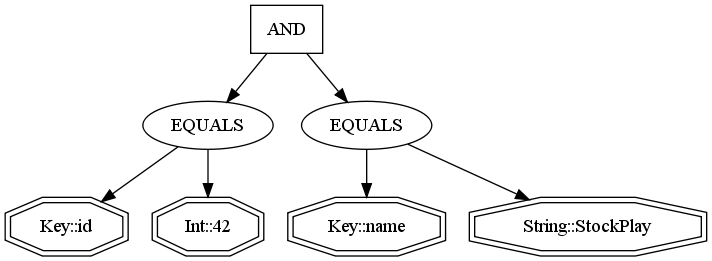
\includegraphics[width=\textwidth]{images/realisatie/AST}
	\caption{Abstract Syntax Tree van een voorbeeldfilter.}
\end{figure}


\section{Verwerking}

Nu de semantiek en conversie van onze filter vastligt, konden we starten met de effectieve implementatie ervan: het omzetten naar of toepassen van de filter op een variabele data-backend. Hierbij zijn de twee grote pistes direct duidelijk: toepassing, of omzetting.

\subsection{Lokale toepassing}

Bij deze opzet wordt de filter lokaal toegepast op een binnengehaalde dataset. Het idee hierbij was om alle records op te halen, en de filter dan lokaal een selectie te laten maken. Die selectie, die voldoet aan de eisen die door de gebruiker zijn opgelegd, kan dan teruggestuurd worden.

Hoewel dit idee perfect toepasbaar is bij systemen waar alle data lokaal aanwezig is (zoals een lokale Java data-backend), treden er problemen op als de data enkel remote aanwezig is en lokaal niet gecachet wordt. In dit geval wordt de overhead van het ophalen van alle records veel te groot, zeker toegepast op StockPlay waarbij de Securities-tabel gemakkelijk meer dan duizend records kan bevatten. Hoewel deze evaluatietechniek dus eenvoudiger te implementeren is (het data-backend-specifieke gedeelte is niet meer aanwezig), hebben we door de grote overhead besloten een alternatief te zoeken.

\subsection{Omzetting}

Het alternatief voor een lokale toepassing, is een omzetting van de filter-boom naar een formaat dat geschikt is om op afstand verwerkt te worden. Hierbij is er geen overhead meer aanwezig, maar wordt het geheel een pak complexer daar het moet kunnen omgezet worden naar een specifieke syntax, afhankelijk van de data-backend.

Om dit te kunnen realiseren, hebben we eerst voorzien in een pseudo-abstracte klasse (Convertable, wel instantieerbaar, maar de compile() functie is ``verboden'') die voorziet in een interface en gemeenschappelijke functionaliteit, onder meer voor het verwerken van eventuele parameters. Filter sub-objecten (Condities, Relaties, en Data objecten) breiden vervolgens deze abstracte klasse gepast uit, door niet zozeer functionaliteit toe te voegen, maar louter voorziet in een hi\"erarchie (zo kunnen we later bijvoorbeeld zeggen dat een Condition enkel Data-objecten als argumenten kan aanvaarden).
Het volgend niveau in het Filter model is dat van de effectieve Condities, Relaties, en Datatypes. Een dergelijke klasse (vb ConditionEquals) breidt opnieuw zijn ouder uit, waarbij de toegevoegde functionaliteit bestaat uit het opbouwen van een graaf-subtree (meer hierover later), het specificeren van een functiesignatuur, en het vereisen van een \emph{compile()} functie voor alle implenterende klassen.
Het finale niveau in ons model voorziet in een implementatie van bovenstaande objecten. Zo zal elke Convertable een implementatie moeten hebben voor elke data-backend (bijvoorbeeld sql.ConditionEquals). Via introspectie zal een Convertable at-runtime een correcte implementatie instantieren, wiens \emph{process()} functie dan instaat voor het genereren van een object dat bruikbaar is voor een data-backend (in geval van SQL zal dit een String).

Deze opzet (pseudo-abstracte Convertable objecten die opnieuw een Convertable instanti\"eren die nu wel over een compile() functie beschikt) mag misschien complex lijken, maar het is elementair in het generiek maken van de filters. Aangezien de pseudo-abstracte Convertable objecten rechtstreeks instantieerbaar zijn, kan de Parser een boomstructuur aan dergelijke objecten opstellen zonder weet te hebben van hoe die boom uiteindelijk zal gecompileerd worden. Het is slechts wanneer die aanroep effectief gebeurt, dat elk Convertable object zal opvragen hoe hij gecompileerd moet worden, om zo de juiste Converter op te roepen. Die Converters voorzien ook niet in een \emph{compile()} instructie, omdat die instructie geen parameters vastlegt en dus manueel de private dataleden zou moeten raadplegen om parameters op te halen. Om dit te vermijden hebben we gekozen voor een extra instructie, de \emph{process()} instructie, die w\'el voorziet in een specifieke signatuur om zo verkeerde implementaties van de Convertables te vermijden.

\begin{code}
\begin{verbatim}
id = 42 AND name = "StockPlay"
\end{verbatim}
\caption{Finaal resultaat na omzetting door de SQL-converters.}
\end{code}


\section{Syntaxreferentie}

Zoals reeds beschreven bestaat een filter essenti\"eel uit drie verschillende mogelijke objecten: condities, relaties, en data-objecten. In deze sectie documenteren we die types, en de exacte grammatica die gebruikt moet worden.

\subsection{Operatoren}

\begin{itemize}
\item{Ronde haakjes: wordt gebruikt om conditities en relaties te groeperen om precedentie in te voeren.}
\item{Komma: wordt gebruikt om de argumenten die aan een functie doorgegeven worden, te scheiden (momenteel ongebruikt).}
\end{itemize}

Ronde haakjes zijn nodig wanneer precedentie onduidelijk is. Aangezien er geen niveaus van precendentie gedefini\"eerd zijn tussen verschillende relaties, zullen er altijd haken moeten gebruikt worden wanneer er zich verschillende relaties in eenzelfde filter bevinden. Bij gelijke relaties wordt er echter impliciet linkse-precedentie toegepast, en zijn haken niet vereist.

\begin{code}
\begin{verbatim}
-- door de impliciete linkse-precedentie wordt eerst de
-- id-expressie ge\"evalueerd, vervolgens de age-expressie en
-- tenslotte de name-expressie.
id >= 5 && age >= 10 && name != 'Jan's

\end{verbatim}
\caption{Demonstratie van de impliciete linkse-precedentie.}
\end{code}

\subsection{Datatypes}

De verschillende datatypes kunnen op verschillende manieren opgesteld worden: rechtstreeks, of indirect. De directe manier is echter enkel beschikbaar voor primitieve dataobjecten (integers, floating-point getallen, strings, en sleutels). Hierbij moet de gebruiker louter de waarde van het getal invoegen in de filter, en zal de parser detecteren om welk formaat het gaat.
Indirecte contructie is steeds mogelijk, en is some de enige optie (bij complexere dataobjecten). Hierbij geeft de gebruiker de data in als een \emph{quoted string} (die voldoet aan een vaste grammatica), en zal een karakter na de laatste quote (de \emph{modifier}) indiceren om welk datatype het gaat.

\subsubsection{Sleutels}

Dit speciaal datatype wordt gebruikt om bij een conditie een specifieke kolom te selecteren. Het mag enkel bestaan uit alfabetische karakters (zowel lower- als uppercase), en een \_ symbool. Het wordt niet omringd door aanhalingstekens, indien dit wel het geval zou zijn wordt het gewoon ge\"interpreteerd als een reguliere string.

\begin{code}
\begin{verbatim}
-- id is een sleutel: verwijst naar een specifieke kolom om de
-- gelijkheids-conditie op in te laten werken
id EQUALS 5
\end{verbatim}
\caption{Illustratief gebruik van een sleutel.}
\end{code}

\subsubsection{Tekenreeksen}

Dit datatype stelt een ordinaire string voor, en kan alle karakters omvatten op voorwaarde dat het omsloten wordt door enkele quotes (en mag er dus geen bevatten, \emph{escaping} wordt niet ondersteund. Zoals wellicht zal opvallen lijkt deze notatie sterk op de indirecte constructiemethode die kan gebruikt worden voor andere datatypes, en eigenlijk is het ook zo geimplementeerd: bij afwezigheid van een modifier na de laatste quote wordt die impliciet verondersteld als zijnde een 's', de modifier voor strings.

\begin{code}
\begin{verbatim}
name EQUALS 'Foo'
name EQUALS 'Foo's
\end{verbatim}
\caption{Illustratief gebruik van een tekenreeks.}
\end{code}

\subsubsection{Natuurlijke getallen -- int}

Dit primitief datatype wordt gebruikt om natuurlijk getallen te detecteren, en mag enkel getallen bevatten (eventueel voorafgegaan door een minteken). Het datatype kan rechtstreeks geconstrueerd worden, en bij indirecte constructie wordt het voorgesteld door de modifier 'i'.

\begin{code}
\begin{verbatim}
id EQUALS 5
id EQUALS '5'i
\end{verbatim}
\caption{Illustratief gebruik van een natuurlijk getal.}
\end{code}

\subsubsection{Gehele getallen -- float}

Dit is een uitbreiding van de natuurlijke getallen, en mag zo ook een decimaal punt bevatten om kommagetallen aan te duiden. Het datatype kan rechtstreeks geconstrueerd worden, en bij indirecte constructie wordt het voorgesteld door de modifier 'f'.

\begin{code}
\begin{verbatim}
cash EQUALS 123.45
cash EQUALS '123.45'f
\end{verbatim}
\caption{Illustratief gebruik van een geheel getal.}
\end{code}

\subsubsection{Datums -- date}

Dit is een voorbeeld van een complex type dat enkel kan geconstrueerd worden via de indirecte methode, gebruik makend van modifier 'd'. Aangezien datums op verschillende manieren kunnen voorgesteld worden, accepteren we enkel volgende methoden (gestandaardiseerd in ISO 8601):
\begin{itemize}
\item{YYYY-MM-DD: 2010-04-07}
\item{YYYY-MM-DD'T'HH:MM'Z': 2010-04-07T05:56Z}
\end{itemize}

Uren zijn steeds in 24-uurs formaat, gespecificeerd in de UTC-tijdzone. Bij afwezigheid van het uur (vb. in YYYY-MM-DD), wordt dit impliciet ingesteld op '00:00' (middernacht), en zal ook zo in de database-backend verwerkt worden. De converters hebben dus geen weet van de manier waarop de datum ingegeven is (al dan niet met gespecificeerd uur).

\begin{code}
\begin{verbatim}
date EQUALS '2010-04-07'd
date EQUALS '2010-04-07T16:01Z'd
\end{verbatim}
\caption{Illustratief gebruik van een datum.}
\end{code}

\subsubsection{Reguliere expressies -- regex}

Dit complex datatype wordt steeds gebruikt in combinatie met de LIKE operator, en kan enkel geconstrueerd worden via de indirecte methode, gebruik makend van de modifier 'r'. Dit datatype ondersteund als enige ook extra modifiers, die het gedrag van de reguliere expressie verfijnen. De volgende extra modifiers worden ondersteund:
\begin{itemize}
\item 'i' modifier: zorgt dat de reguliere expressie case-insensitive werkt
\end{itemize}

\begin{code}
\begin{verbatim}
name LIKE '^j*n$'ri
\end{verbatim}
\caption{Illustratief gebruik van een reguliere expressie.}
\end{code}

\subsection{Condities}

Een conditie wordt gebruikt om een specifieke vergelijkingsoperatie toe te passen op een kolom, zodat er een selectie gebeurd op basis van deze conditie. De mogelije condities (met tussen haken de signatuur) zijn:

\begin{itemize}
\item == of EQUALS: vereist dat twee velden identiek zijn [Key, *]
\item != of NOTEQUALS: vereist dat twee velden verschillend zijn [Key, *]
\item $>$ of GREATHERTHAN: vereist dat het ene veld groter is dan het andere [Key, *]
\item $<$ of LESSTHAN: vereist dat het ene veld kleiner is dan het andere [Key, *]
\item $>$= of GREATHERTHANOREQUAL: vereist dat het ene veld strikt groter is dan het andere [Key, *]
\item $<$= of LESSTHANOREQUAL: vereist dat het ene veld strikt kleiner is dan het andere [Key, *]
\item =\textasciitilde of LIKE: vereist dat het ene veld voldoet aan de string (met wildcards) in het tweede veld [Key, String]
\item !\textasciitilde of NOTLIKE: vereist dat het ene veld verschilt van de string (met wildcards) in het tweede veld [Key, String]
\end{itemize}

\subsection{Relaties}

Relaties dienen om verschillende condities aan elkaar te schakelen, en het resultaat op een specifieke wijze te interpreteren.

\begin{itemize}
\item \&\& of AND
\item $||$ of OR
\end{itemize}

\subsection{Functies}

Momenteel zijn er nog geen functies gedefini\"eerd in de parser, maar de infrastructuur is er op voorzien. Mits een eenvoudige uitbreiding van de tokenizer kan er zelf gebruik gemaakt worden van functies met een variabel aantal argumenten.


